
\chapter{Results}

\subsection{Charge Bin studies}

All of the studies were performed on the RH0017 module, which is a $1 \times 2$ CROC module with an HPK bias-dot $100 \times 25~\mu\text{m}^2$ sensor, where the shorter pitch corresponds to the $Y$ direction and the longer to the $X$ direction. The sensor layout has already been shown in Figure~\ref{fig:xtalk_layout}. The sensor is planar and non-irradiated. During data taking, the module was operated using chiller cooling only, following damage to the cold box due to a Peltier temperature excursion. The high-voltage bias was set to $-100$\,V. All the presented data correspond to a threshold of 1000 electrons.

The main purpose of the charge Bin studies is to better understand the effect of delta rays on the DUT and telescope resolution. If the effect is noticeable and significant, it could justify excluding such tracks from the general alignment procedure. This could potentially improve the telescope alignment by removing tracks associated with secondary particle production, which degrade the precision of the data.

The charge distribution is typically Landau-like, with delta-ray tracks contributing to the high-charge tail of the distribution. More specifically:
\begin{itemize}
    \item \textbf{Bin 3 (Low charge)}: $0 < Q \leq 0.85\,Q_a$
    \item \textbf{Bin 2 (Below average)}: $0.85\,Q_a < Q \leq Q_a$
    \item \textbf{Bin 1 (Above average)}: $Q_a < Q \leq 1.5\,Q_a$
    \item \textbf{Bin 0 (High charge / delta-ray candidates)}: $Q > 1.5\,Q_a$
\end{itemize}
\noindent
where \( \mathbf{Q_a} \) denotes the mean (average) detected charge across all clusters or see the Figure~\ref{fig:charge_bins}.

\begin{figure}[H]
    \centering
    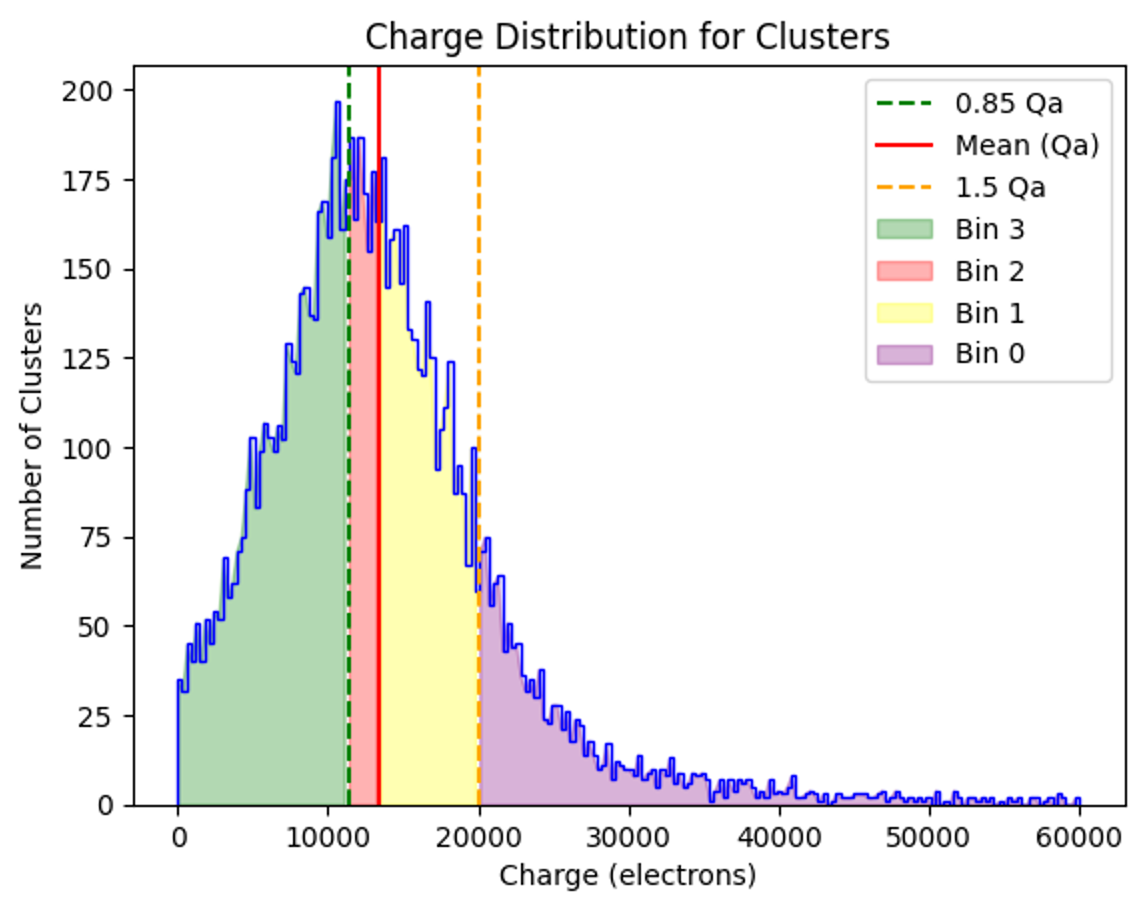
\includegraphics[width=0.7\textwidth]{images/Bins.png}
    \caption{Representation of the studied charge Bins with respect to \( Q_a \), the mean detected charge.}
    \label{fig:charge_bins}
\end{figure}

Resolution for the clusters of cluster size 2 is always superior to that for the clusters of other cluster sizes due to charge sharing. In this way, the track was traversing the DUT closer to the pixel edge, and the predicted position difference is smaller than when detected anywhere within even 1 pixel. It is also expected that for lower charge Bins (delta-ray candidates), the clusters formed are larger than for other charges, which will lead to having more clusters with large cluster sizes, like in Bin 0. Thus, comparing the residual distributions for cluster size 1 and cluster size 3 was considered to be helpful. The results obtained are presented in Figure~\ref{fig:resolution_size_1&3}. The residual is then approximated on all the planes of the telescope, with measurements taken using the DUT. Intuitively, the residual for cluster size 1 should be better, and this was confirmed by the results, even though the difference is not as significant.

\begin{figure}[H]
    \centering
    \begin{subfigure}[t]{0.485\textwidth}
        \centering
        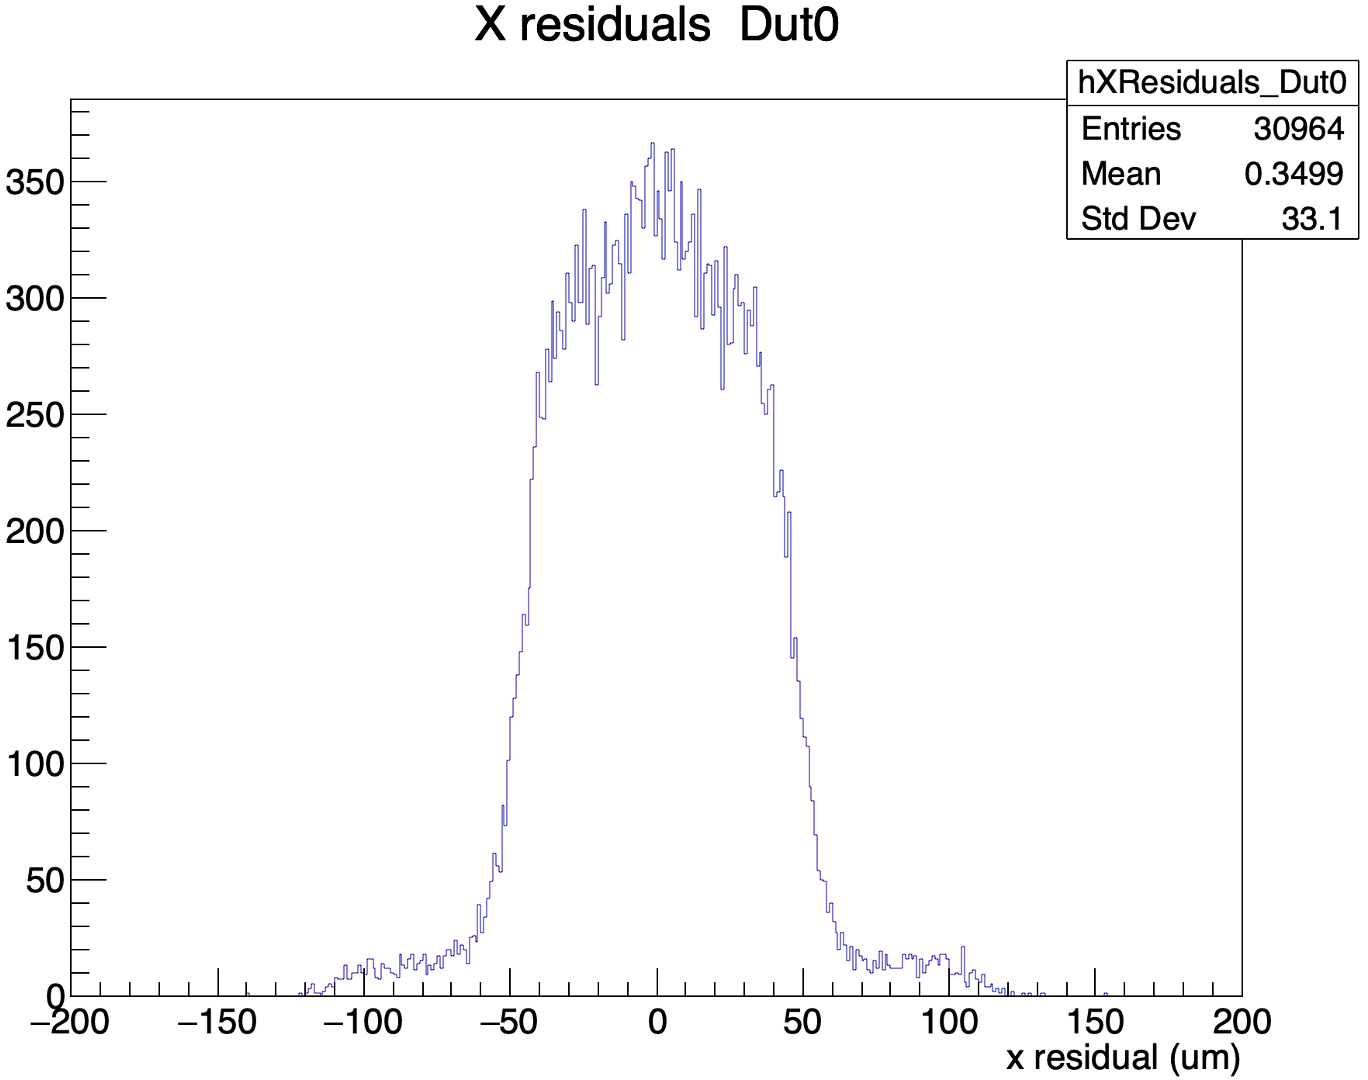
\includegraphics[width=\textwidth]{images/XRes_13planes.png}
        \caption{}
        \label{fig:dist_a}
    \end{subfigure}
    \hfill
    \begin{subfigure}[t]{0.45\textwidth}
        \centering
        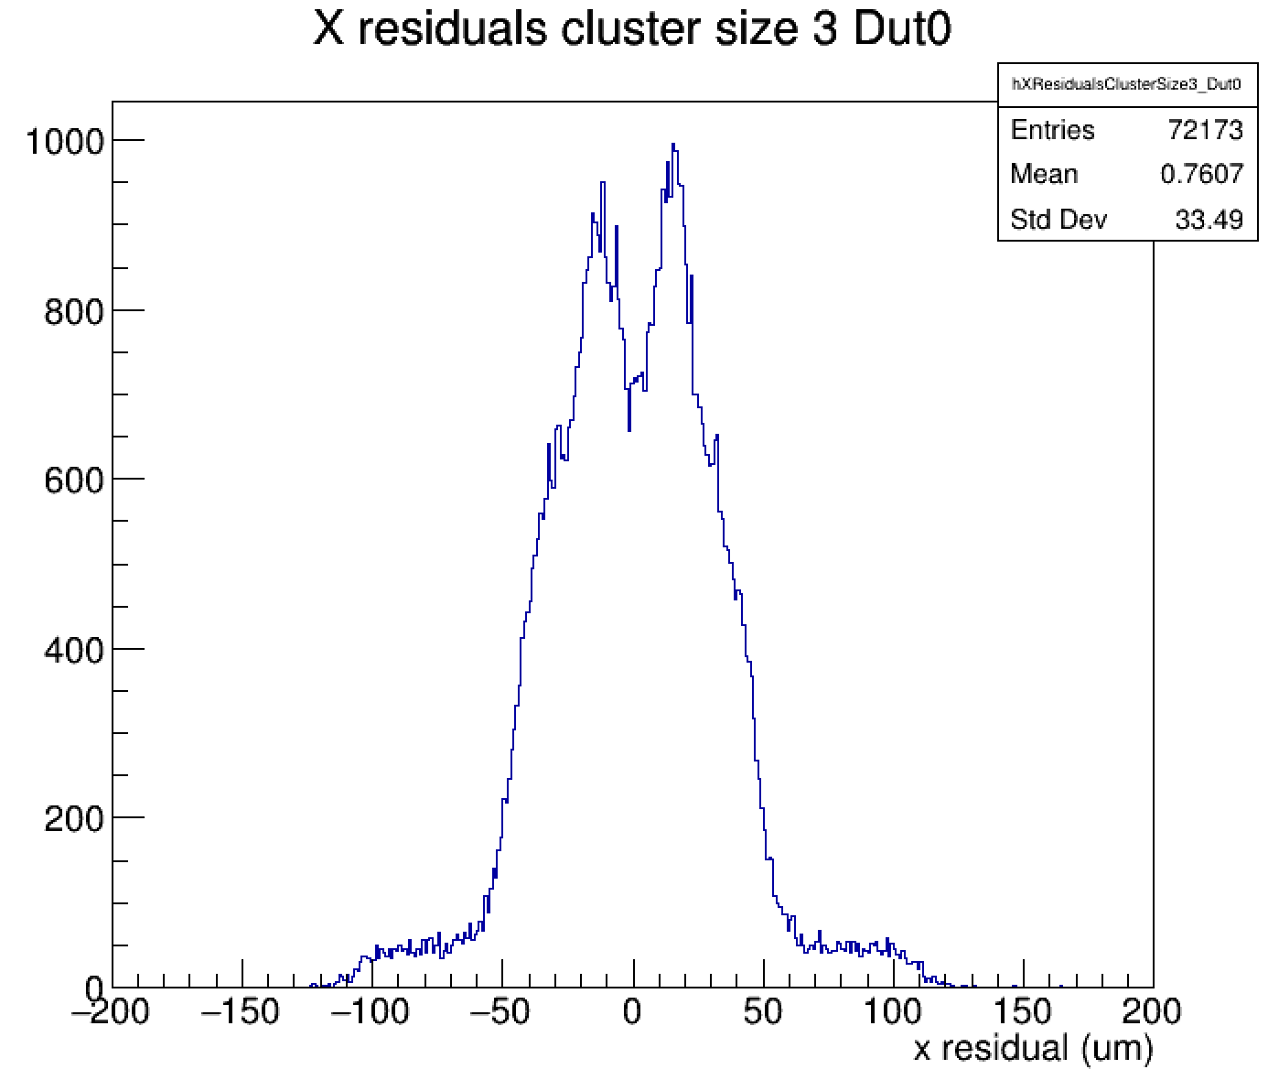
\includegraphics[width=\textwidth]{images/XRes_size3.png}
        \caption{}
        \label{fig:dist_b}
    \end{subfigure}

    \vspace{0.5cm}

    \begin{subfigure}[t]{0.5\textwidth}
        \centering
        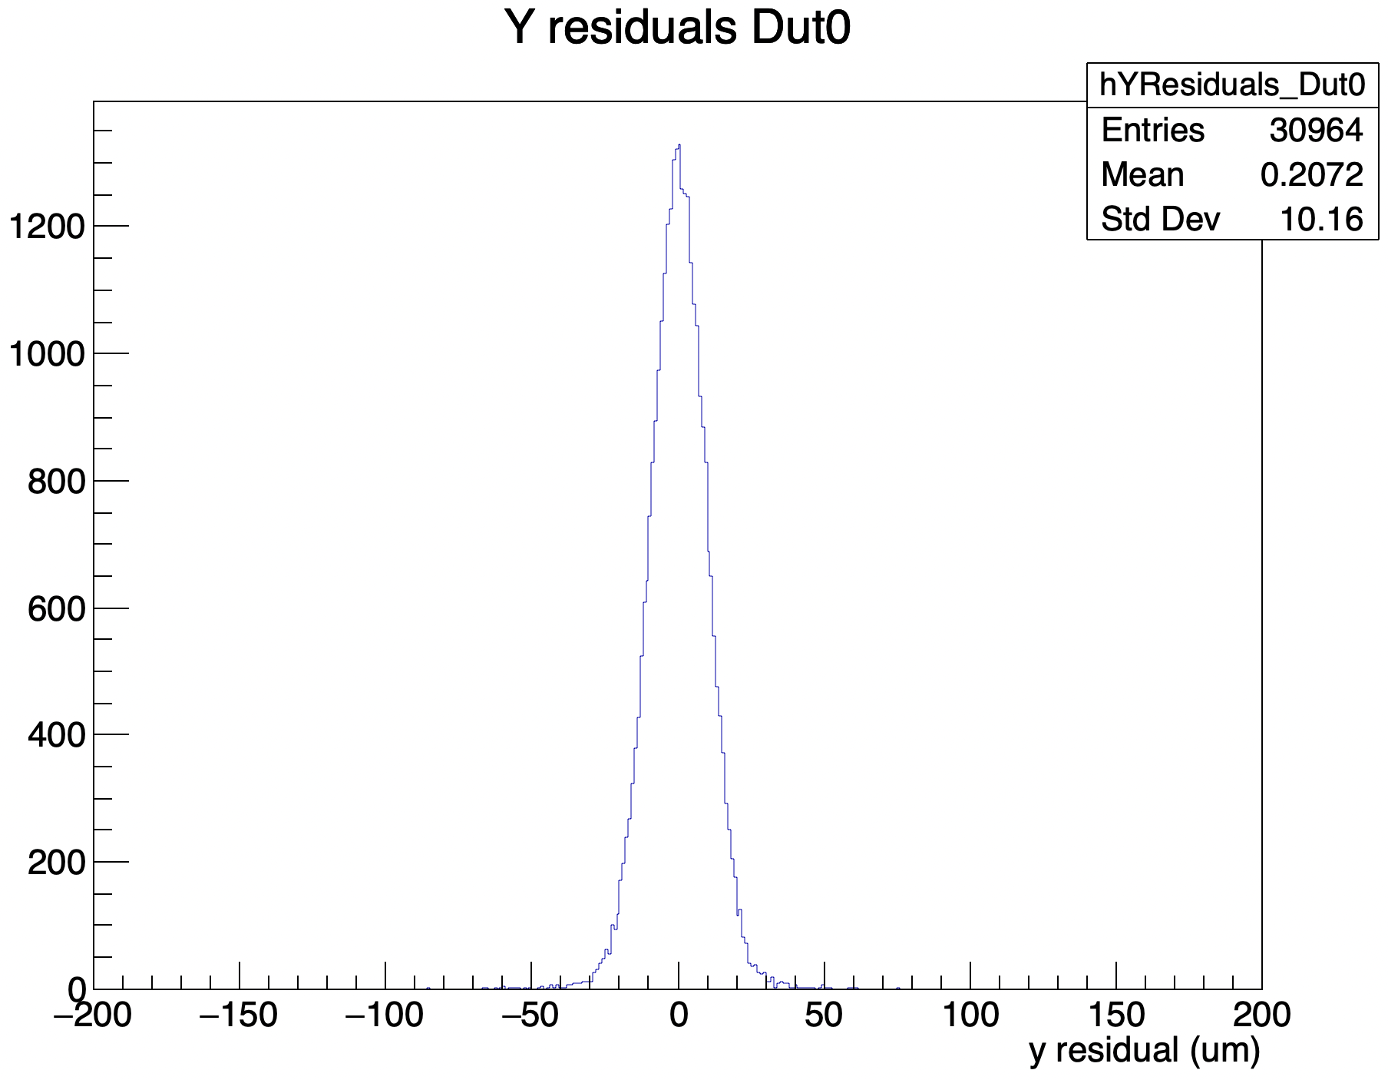
\includegraphics[width=\textwidth]{images/YRes_13planes.png}
        \caption{}
        \label{fig:dist_c}
    \end{subfigure}
    \hfill
    \begin{subfigure}[t]{0.45\textwidth}
        \centering
        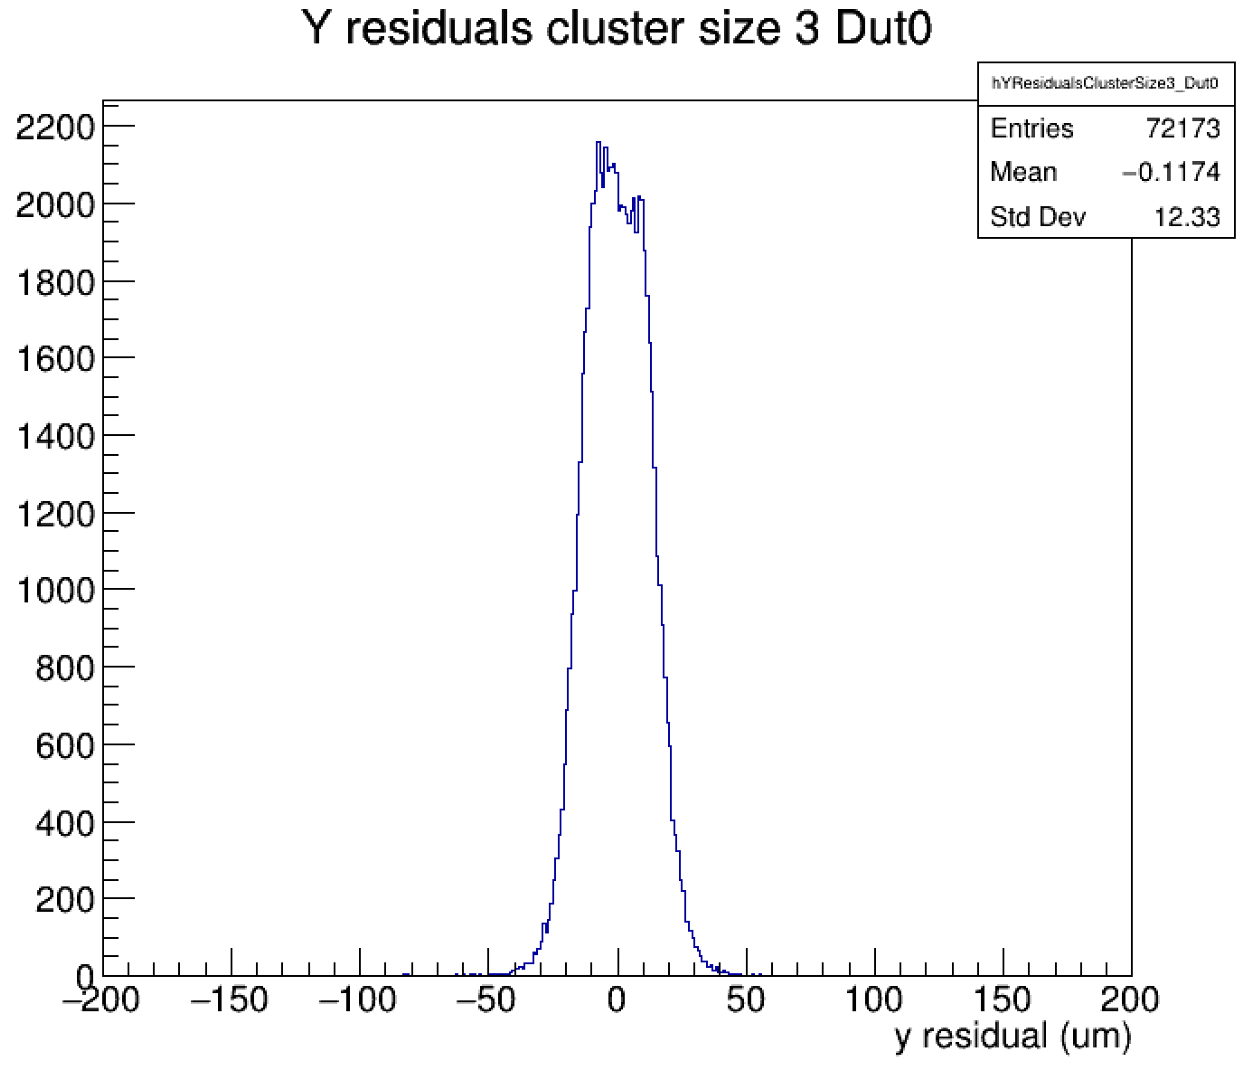
\includegraphics[width=\textwidth]{images/YRes_size3.png}
        \caption{}
        \label{fig:dist_d}
    \end{subfigure}

    \caption{Residual distributions in the X direction for cluster sizes 1 and 3 are shown in (a) and (b), respectively. Corresponding residuals in the Y direction for cluster sizes 1 and 3 are presented in (c) and (d).}
    \label{fig:resolution_size_1&3}
\end{figure}

In addition for the further investigation was important to look at the cluster size distribution for the different charge Bins. The results are shown in Figure~\ref{fig:cluster_bins_vs_size}. The results show that the cluster sizes increase as the charge Bin decreases. This supports the expectation, as delta-ray candidates (Bin 0) are anticipated to produce larger clusters than other charge Bins. Additionally, for the remaining charge Bins, the cluster sizes also increase consistently.

\begin{figure}[H]
    \centering
    \begin{subfigure}[t]{0.45\textwidth}
        \centering
        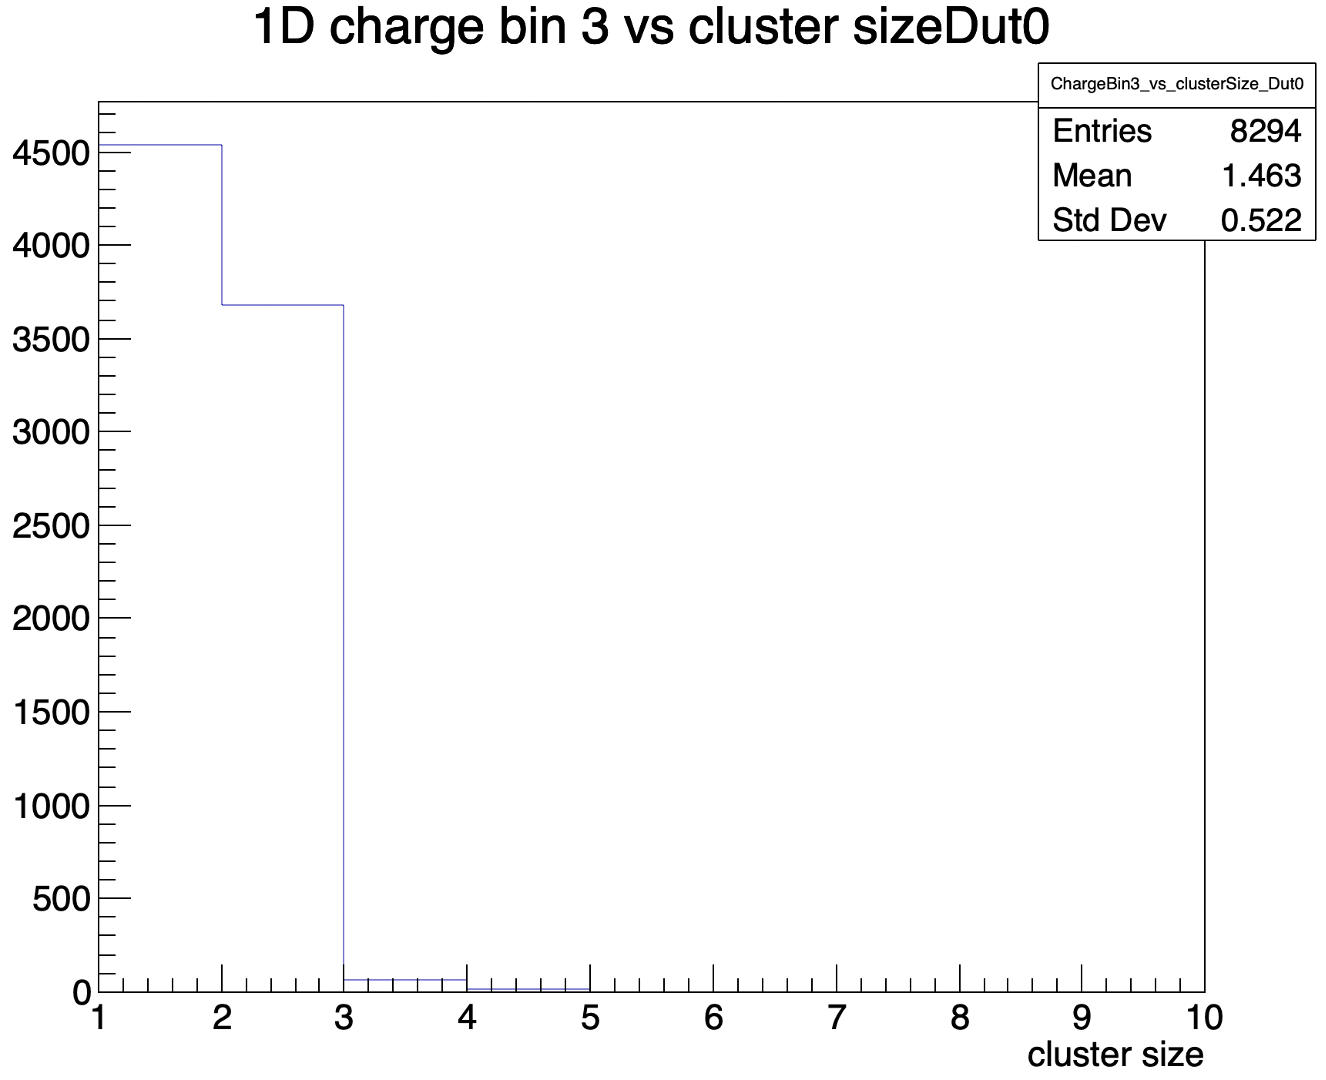
\includegraphics[width=\textwidth]{images/chargeBin3_us_clsize.png}
        \caption{}
        \label{fig:dist_a}
    \end{subfigure}
    \hfill
    \begin{subfigure}[t]{0.45\textwidth}
        \centering
        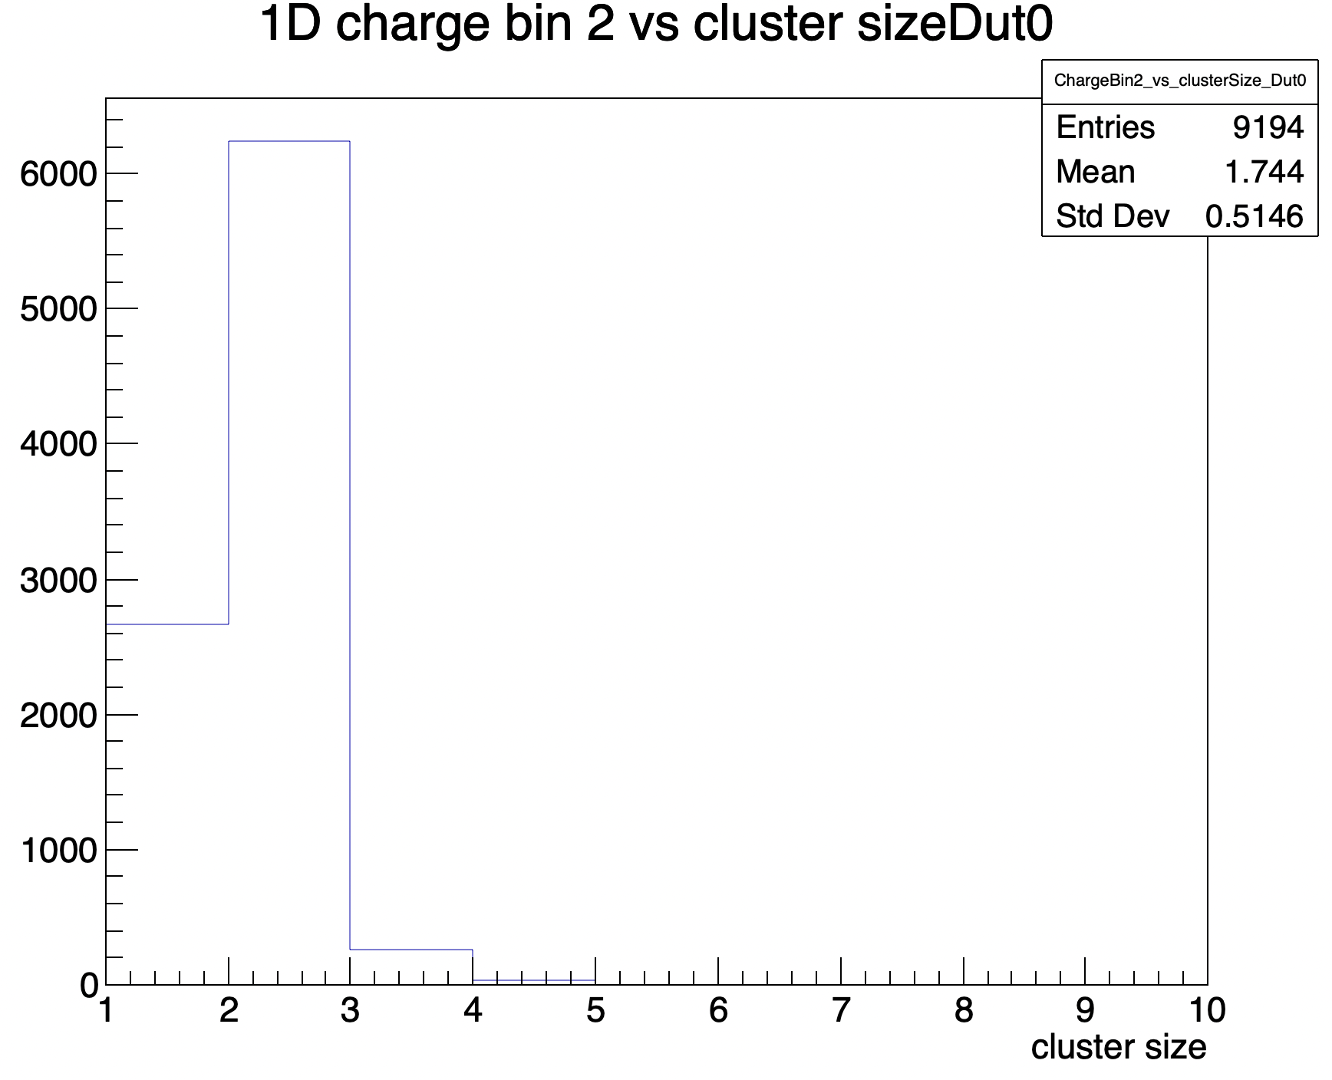
\includegraphics[width=\textwidth]{images/ClusBin2_us_clus_size.png}
        \caption{}
        \label{fig:dist_b}
    \end{subfigure}

    \vspace{0.5cm}

    \begin{subfigure}[t]{0.45\textwidth}
        \centering
        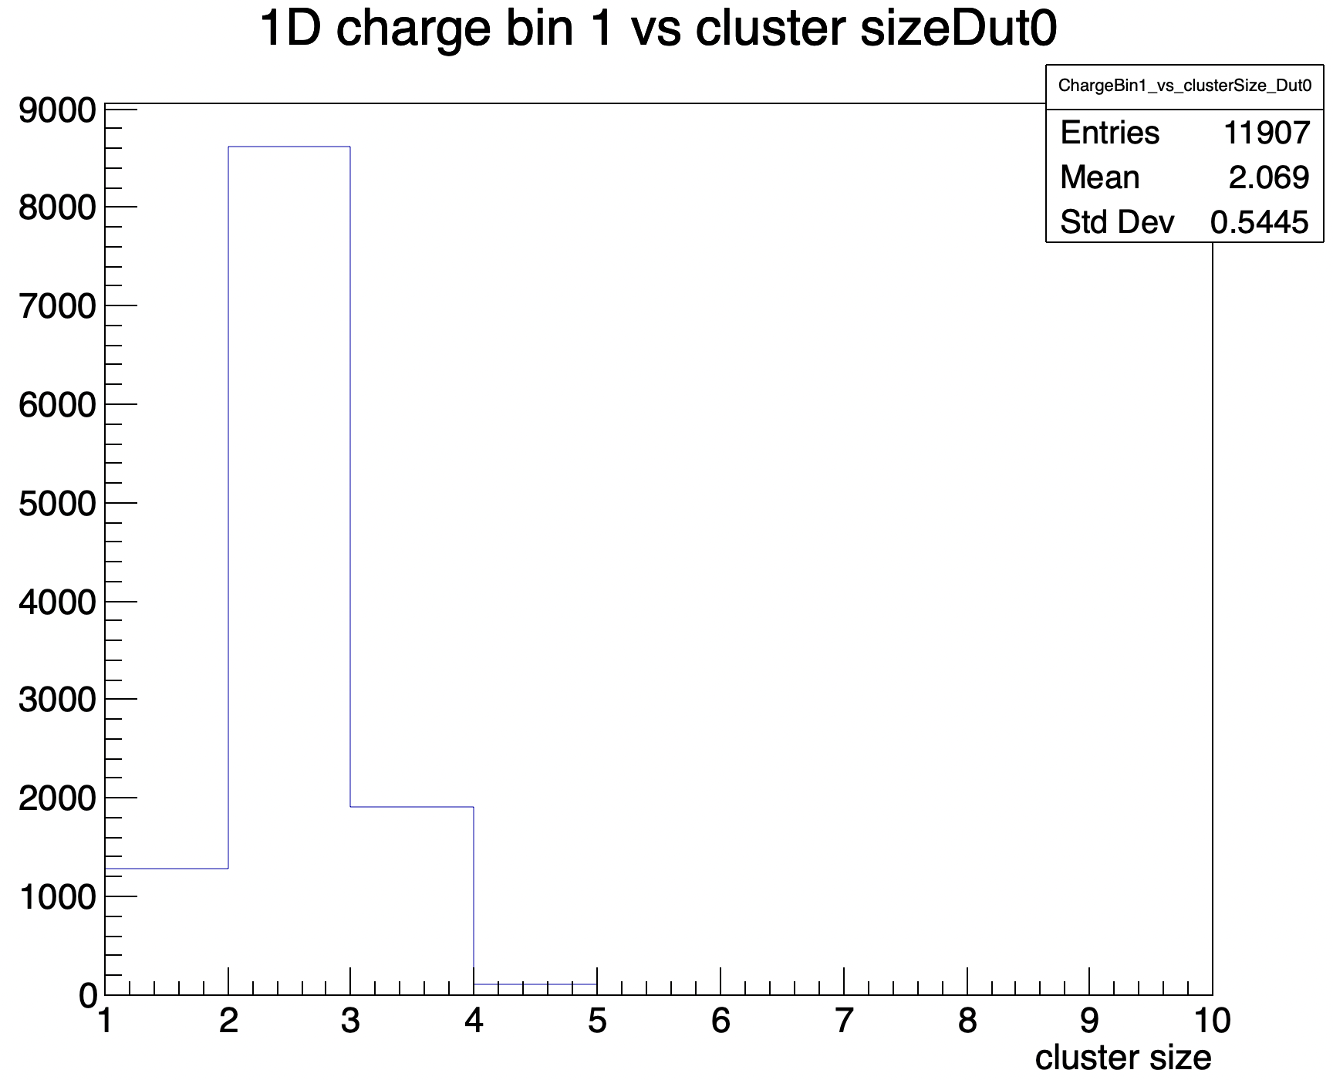
\includegraphics[width=\textwidth]{images/ChargeBin1_us_clus_size.png}
        \caption{}
        \label{fig:dist_c}
    \end{subfigure}
    \hfill
    \begin{subfigure}[t]{0.45\textwidth}
        \centering
        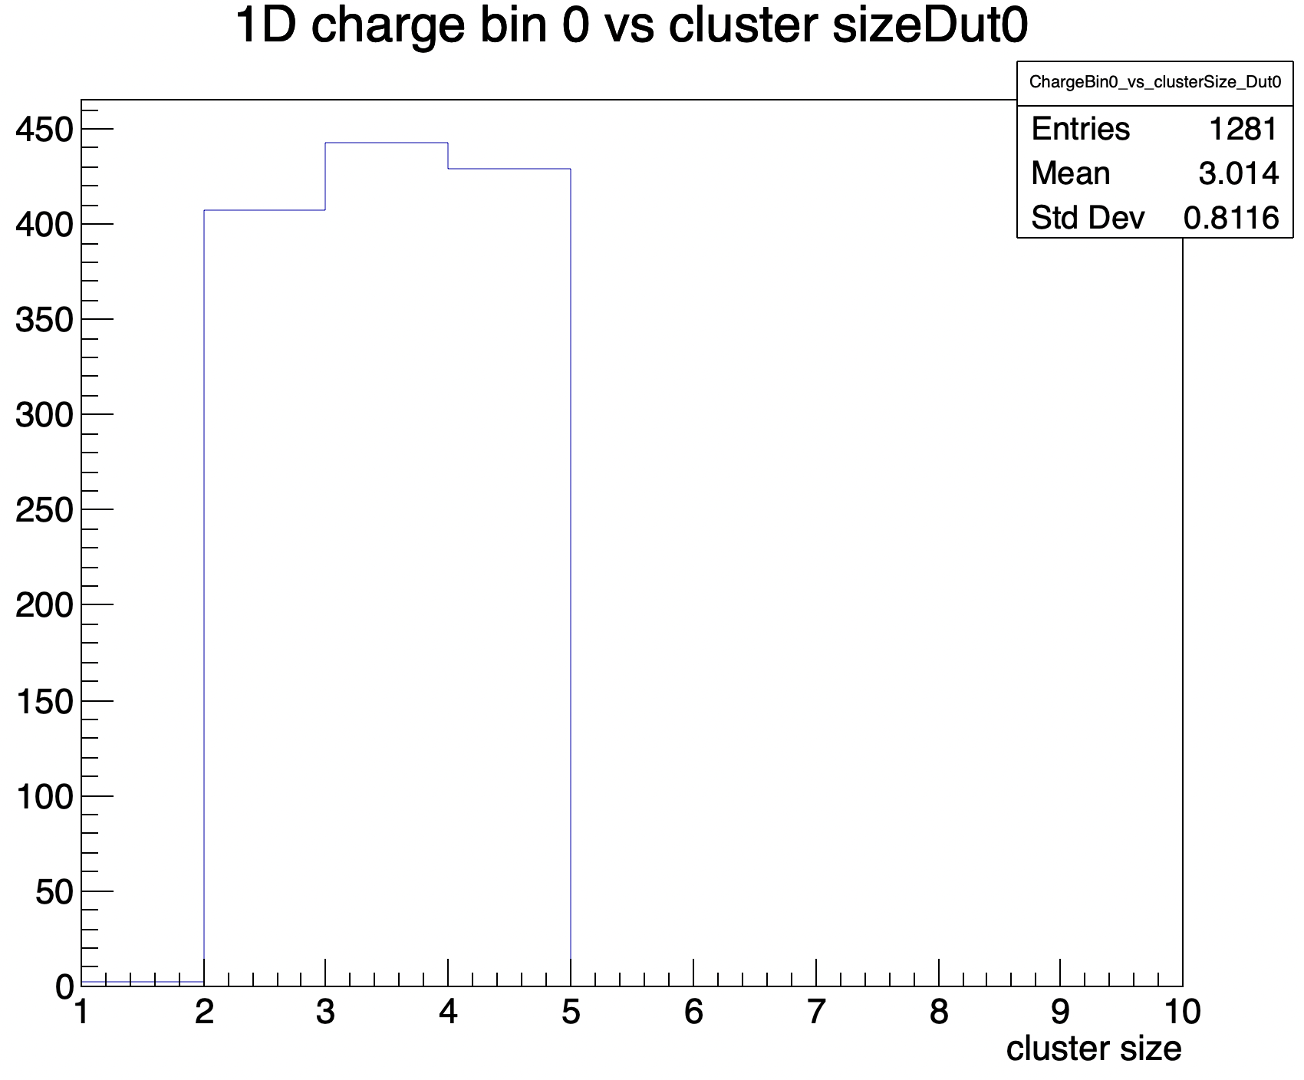
\includegraphics[width=\textwidth]{images/ChargeBin0_us_clus_size.png}
        \caption{}
        \label{fig:dist_d}
    \end{subfigure}

    \caption{Charge Bins versus cluster size of produced clusters for Bin~3 (a), Bin~2 (b), Bin~1 (c), and Bin~0 (d), respectively where the cluster size is defined as the number of pixels in a cluster.}
    \label{fig:cluster_bins_vs_size}
\end{figure}

In order to investigate whether the exclusion of charge Bin 0 improves the resolution, the X and Y predicted errors were examined. By default, the alignment previously required each track to pass through at least 13 out of 16 planes. Additional results were produced with the stricter condition that each individual track must pass through all four pixel planes. The track reconstruction was performed using hits from all pixel planes, and the predicted errors were evaluated at the DUT. All configurations were compared, and the results are shown in Figure~\ref{fig:X_Y_Predicted_Errors}. The measurement precision improved significantly when tracks were required to pass through all pixel planes. However, although the precision also improved after excluding Bin 0 tracks (delta-ray candidates), the difference was relatively minor.

\begin{figure}[H]
    \centering

    \begin{subfigure}[b]{0.3\textwidth}
        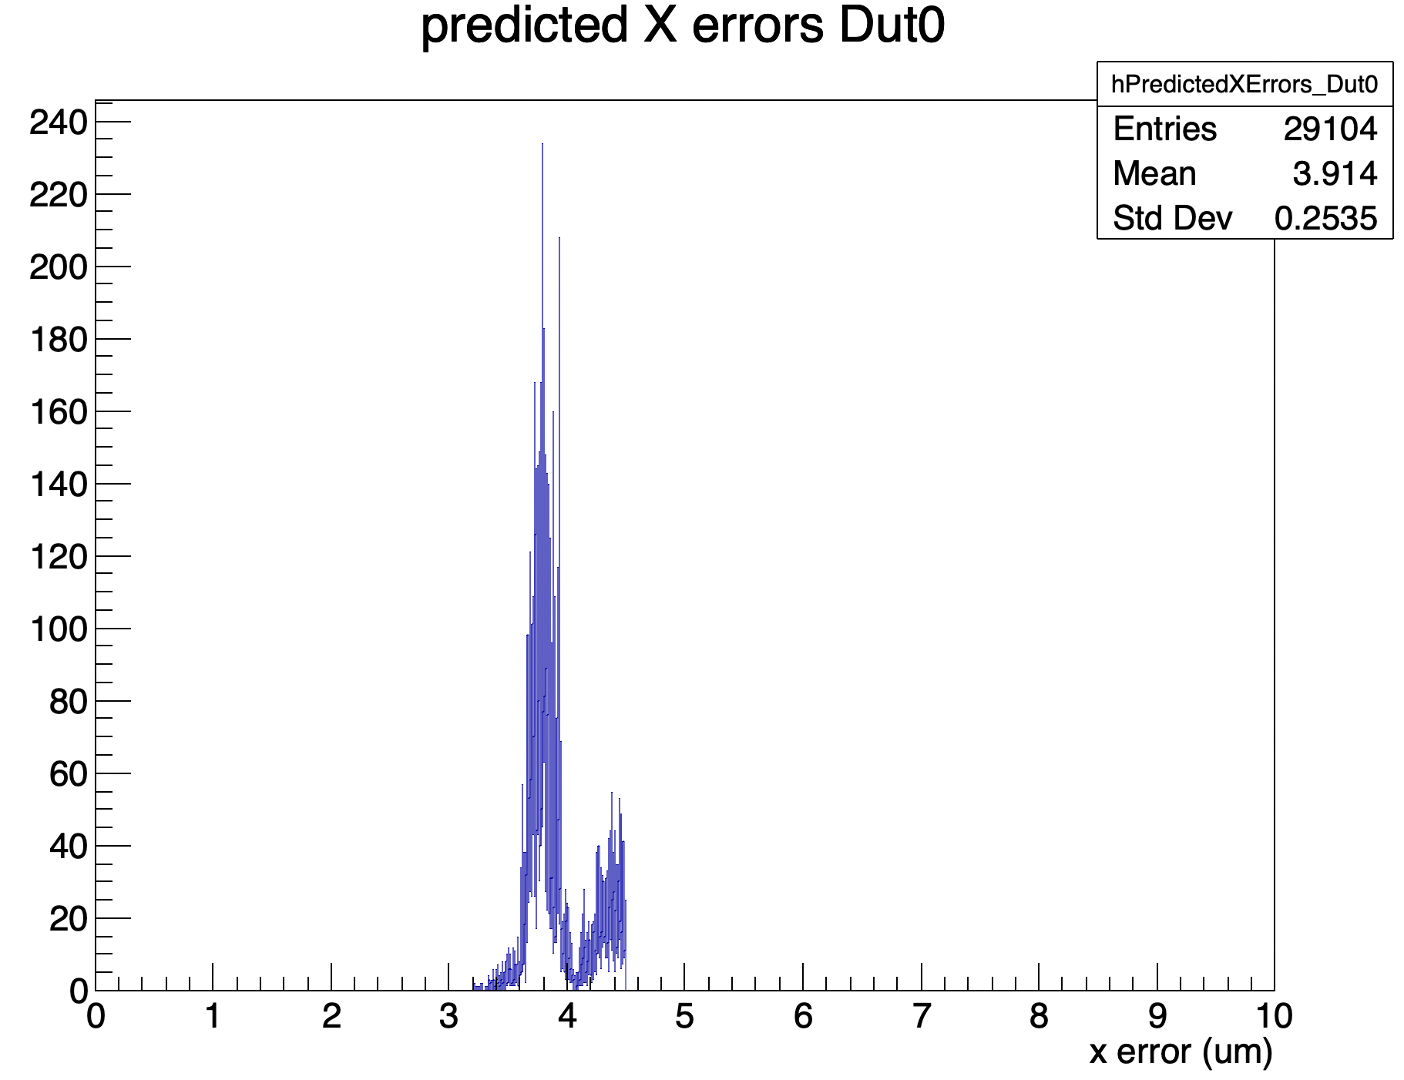
\includegraphics[width=\textwidth]{images/XPredError_13planes.png}
        \caption{}
    \end{subfigure}
    \hfill
    \begin{subfigure}[b]{0.33\textwidth}
        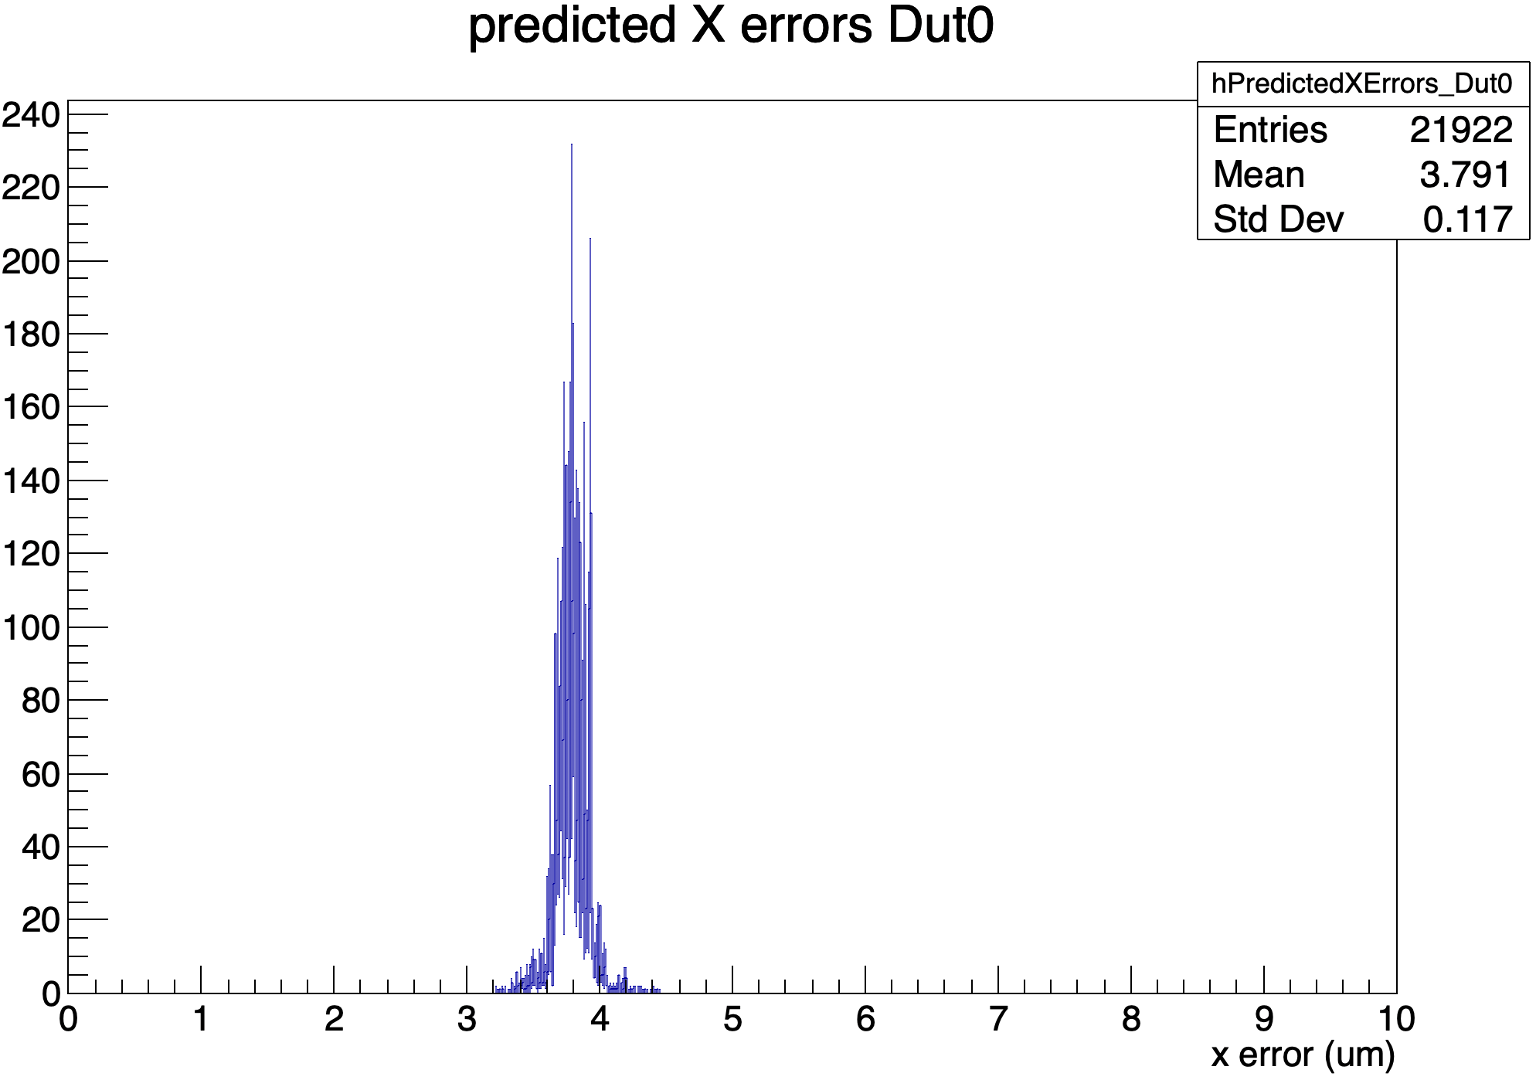
\includegraphics[width=\textwidth]{images/XPredError_4pixel.png}
        \caption{}
    \end{subfigure}
    \hfill
    \begin{subfigure}[b]{0.3\textwidth}
        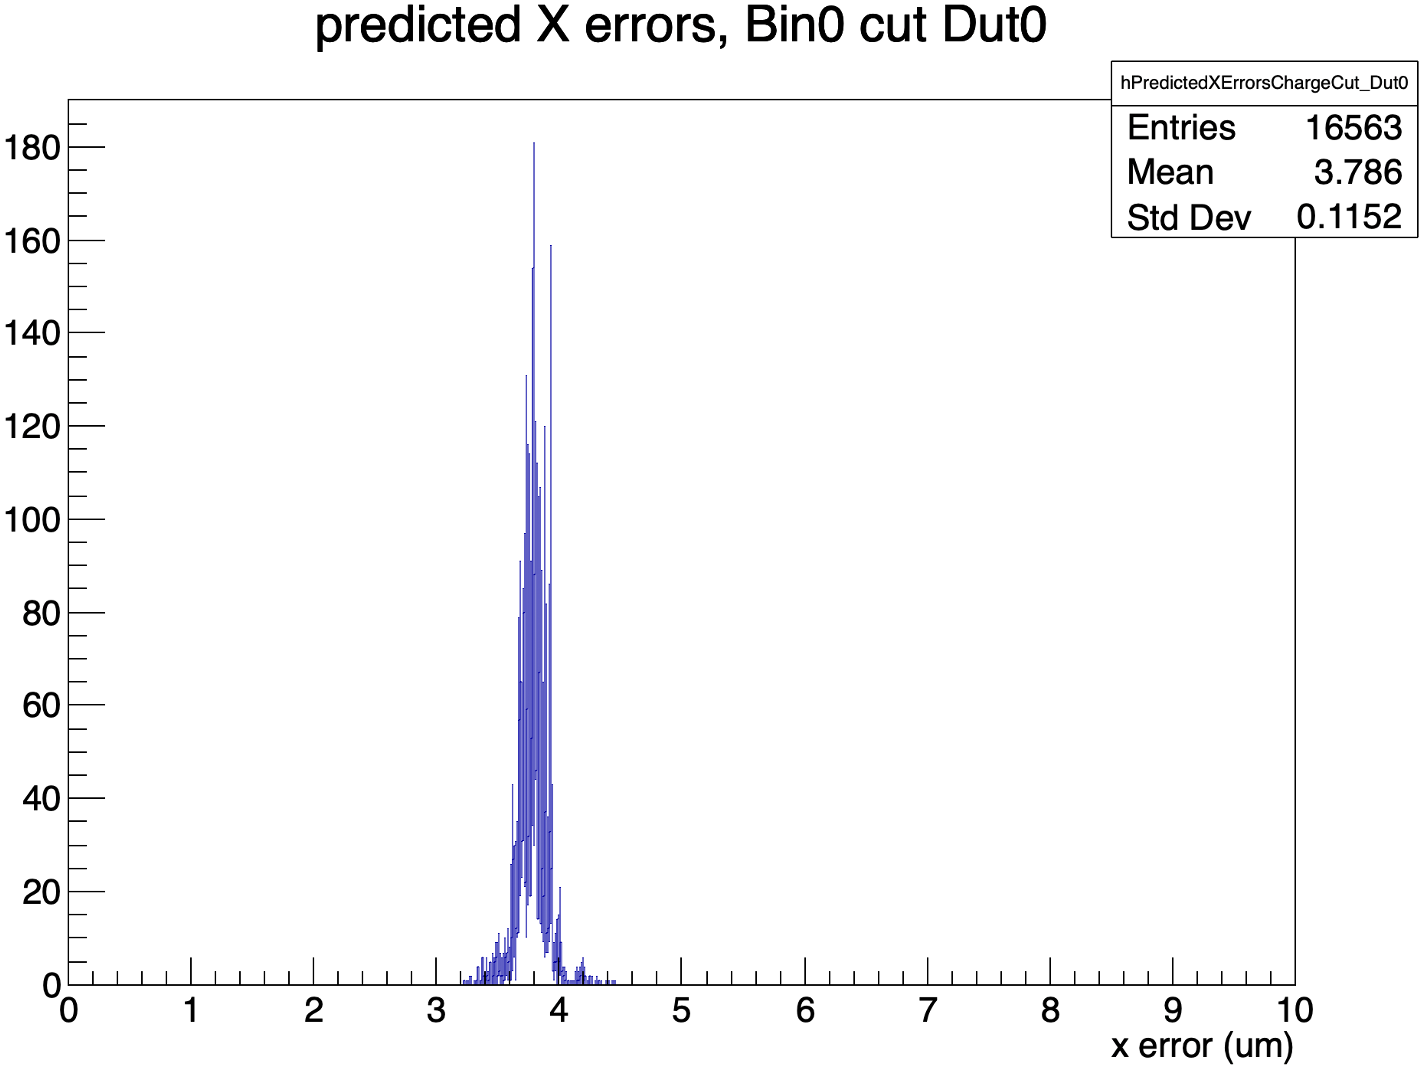
\includegraphics[width=\textwidth]{images/XPredError_4pixel_noBin0.png}
        \caption{}
    \end{subfigure}

    \vspace{0.5cm} % optional spacing between rows

    \begin{subfigure}[b]{0.3\textwidth}
        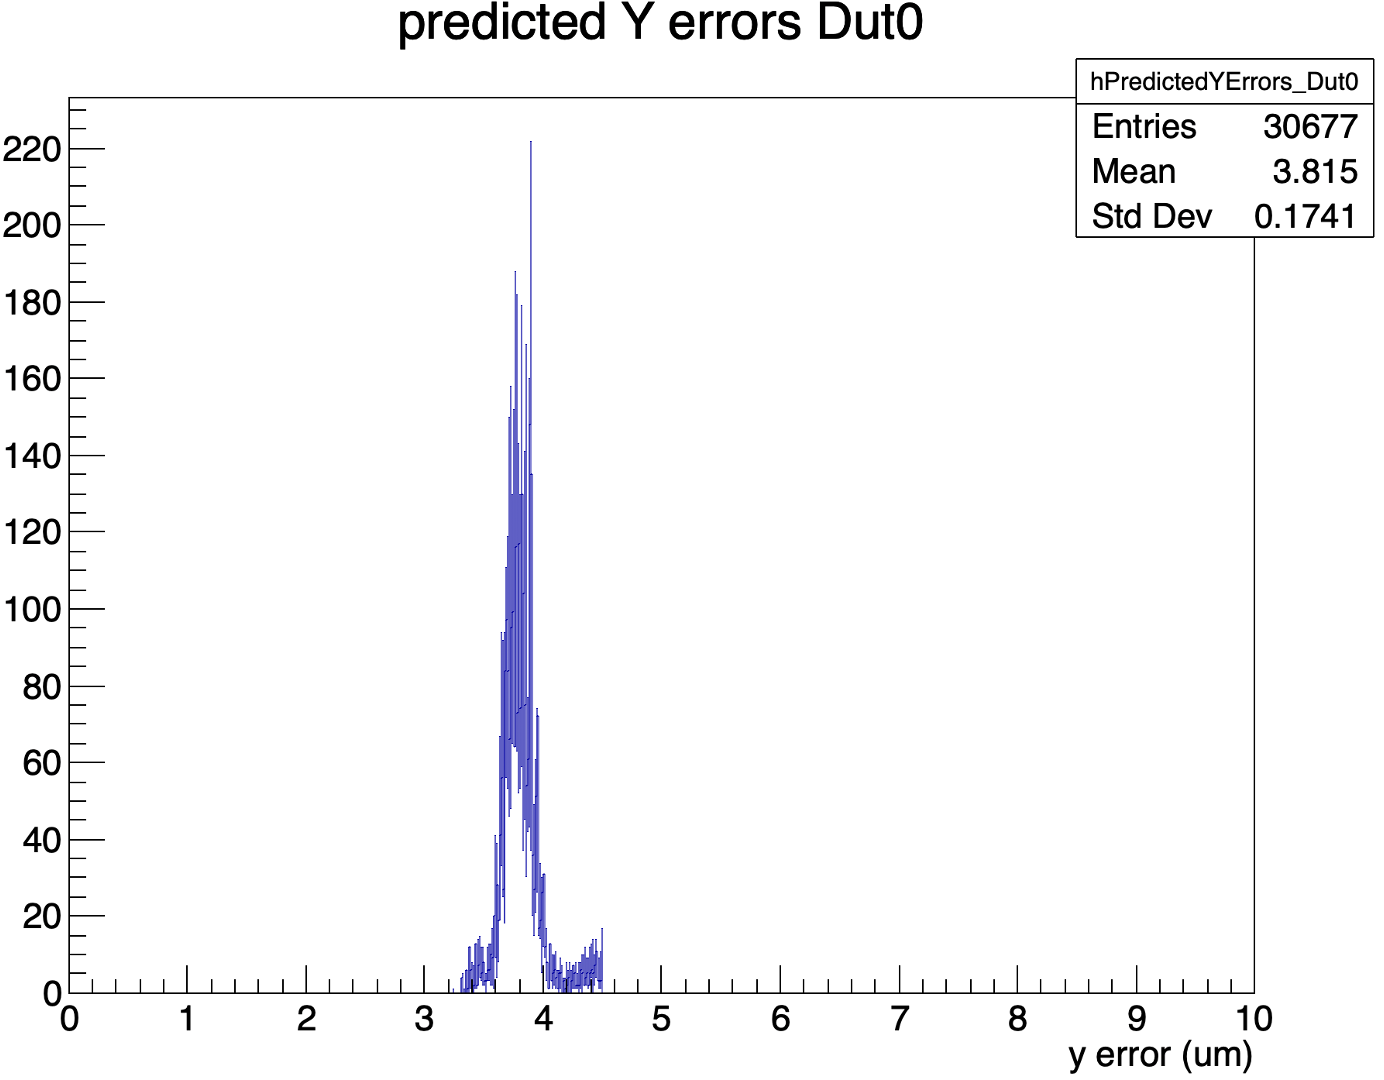
\includegraphics[width=\textwidth]{images/YPredicError_13planes.png}
        \caption{}
    \end{subfigure}
    \hfill
    \begin{subfigure}[b]{0.33\textwidth}
        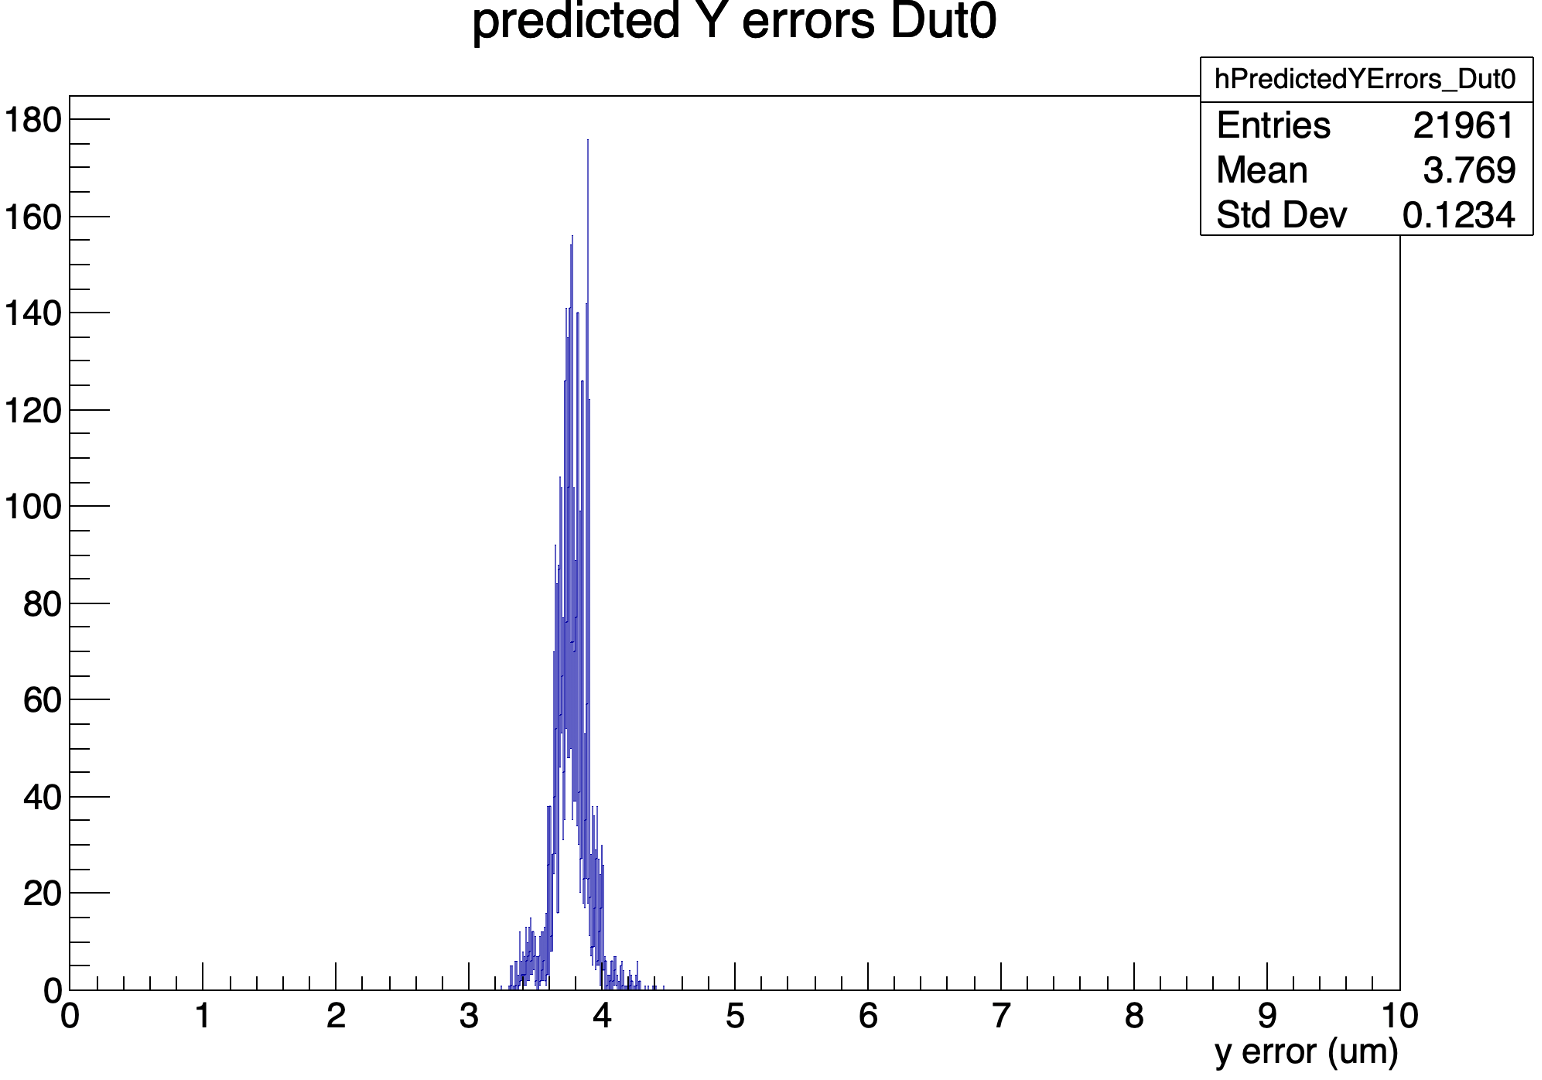
\includegraphics[width=\textwidth]{images/YPredError_4pixel.png}
        \caption{}
    \end{subfigure}
    \hfill
    \begin{subfigure}[b]{0.3\textwidth}
        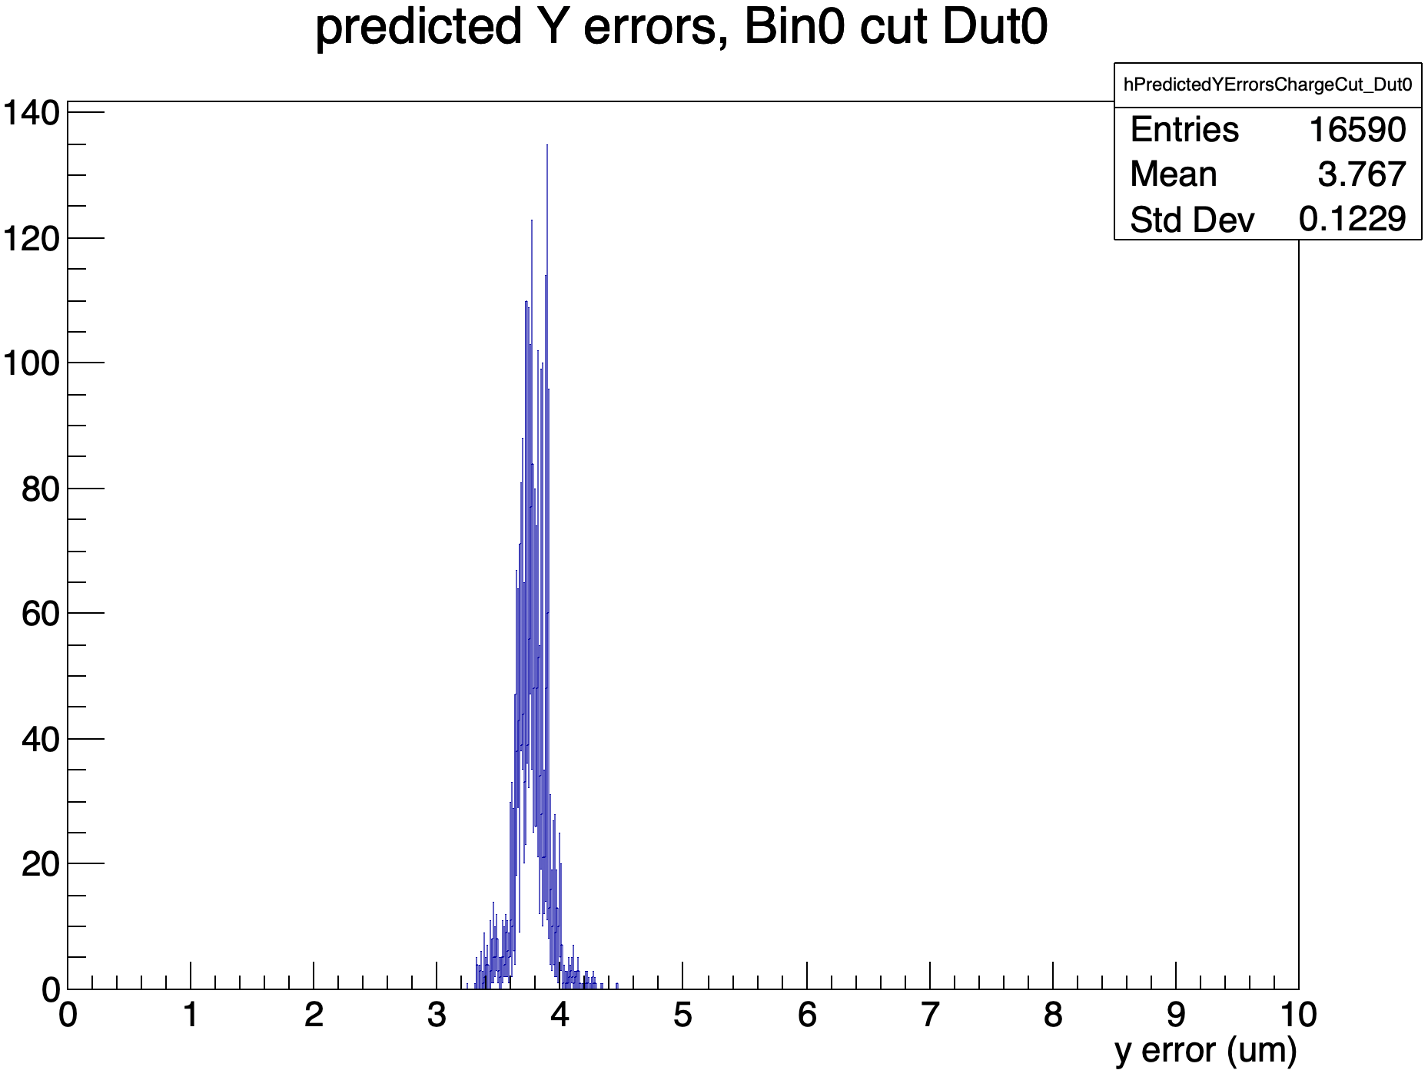
\includegraphics[width=\textwidth]{images/YPredError_4pixel_noBin0.png}
        \caption{}
    \end{subfigure}

    \caption{X predicted error for (a) for 13 planes (b) 4 pixel planes for certain (c) for 4 pixel planes with bin 0 cut and for (d-f) respective values but for Y predicted}
    \label{fig:X_Y_Predicted_Errors}
\end{figure}

Moreover, keeping the same conditions as for the predicted errors, the residuals were also examined. The results are shown in Figure~\ref{fig:X_Y_Residual_planes}. The residuals were calculated as the difference between the predicted and measured positions at the DUT. From the Y residual plots, we observe an improvement when applying the stricter requirement that all four pixel planes be used, as well as a performance enhancement when excluding Bin 0 tracks. However, applying the same restrictions in the X direction had the opposite effect. This requires some further investigation. A similar situation is observed in the residual plots for cluster size 1, shown in Figure~\ref{fig:X_Y_Residual_size_1_planes}.

\begin{figure}[H]
    \centering

    \begin{subfigure}[b]{0.3\textwidth}
        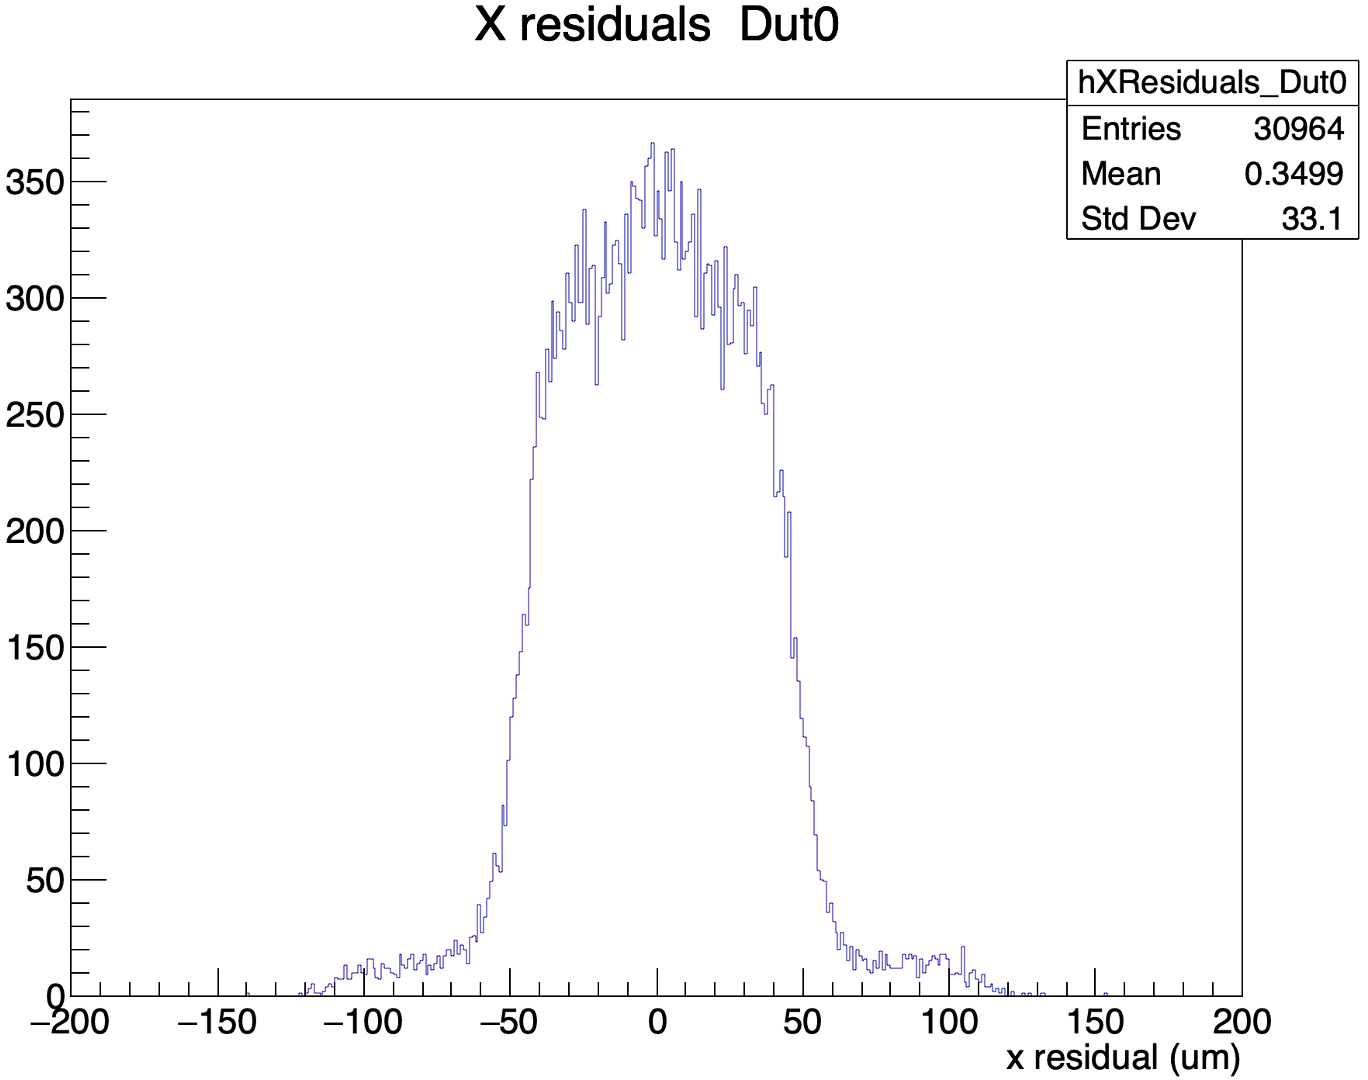
\includegraphics[width=\textwidth]{images/XRes_13planes.png}
        \caption{}
    \end{subfigure}
    \hfill
    \begin{subfigure}[b]{0.33\textwidth}
        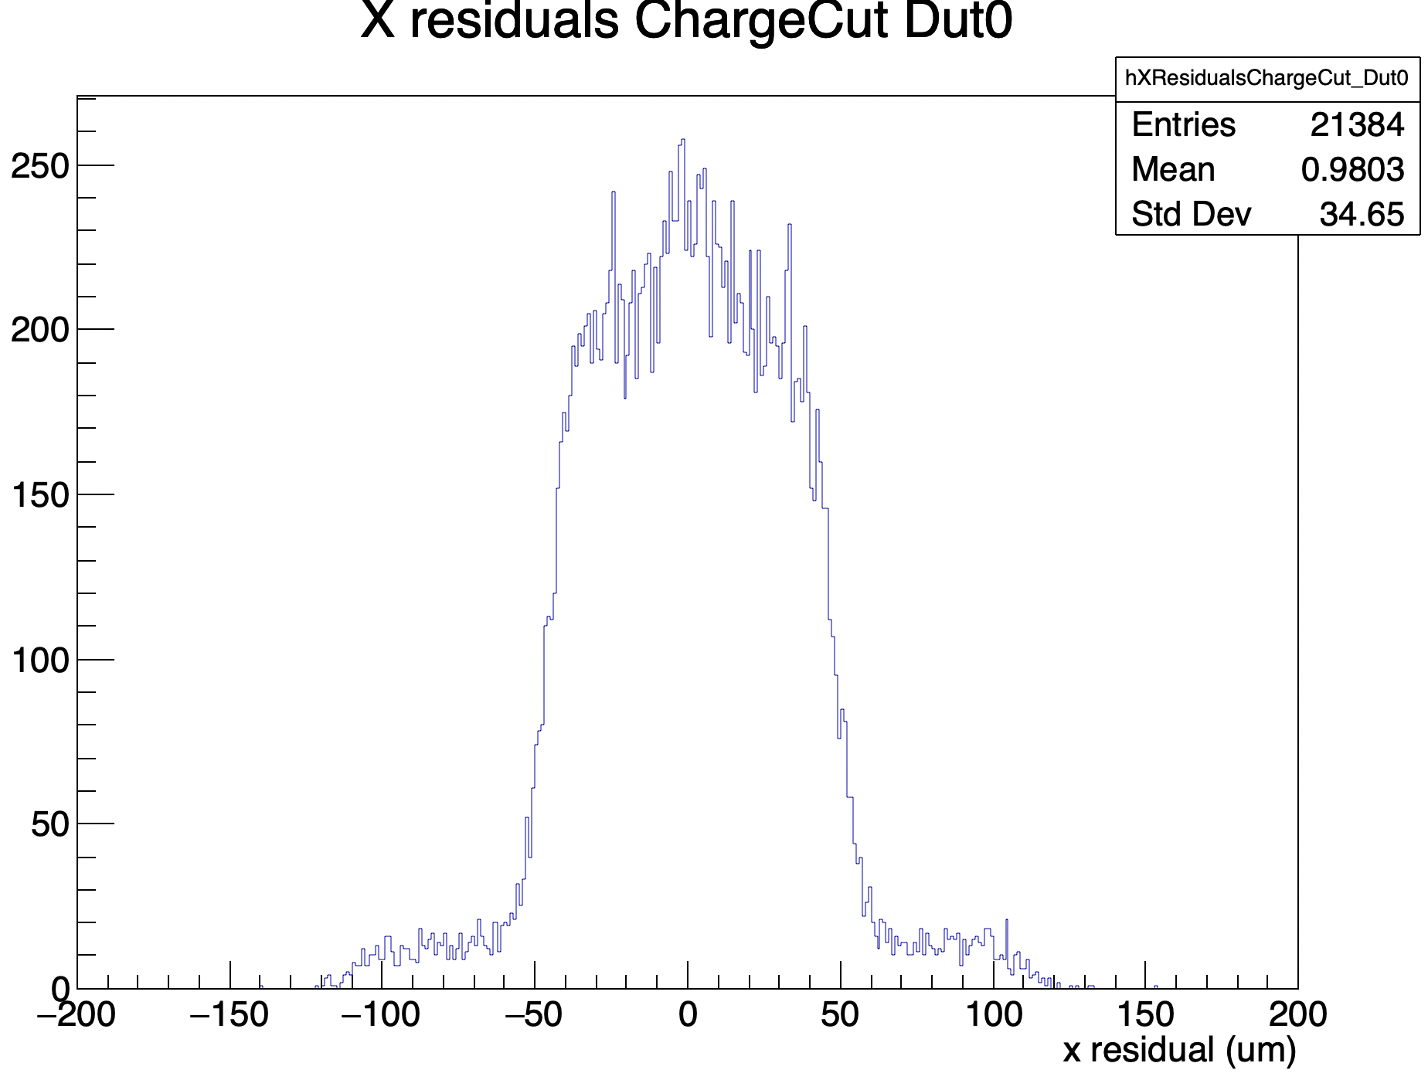
\includegraphics[width=\textwidth]{images/XRes_4pixel.png}
        \caption{}
    \end{subfigure}
    \hfill
    \begin{subfigure}[b]{0.3\textwidth}
        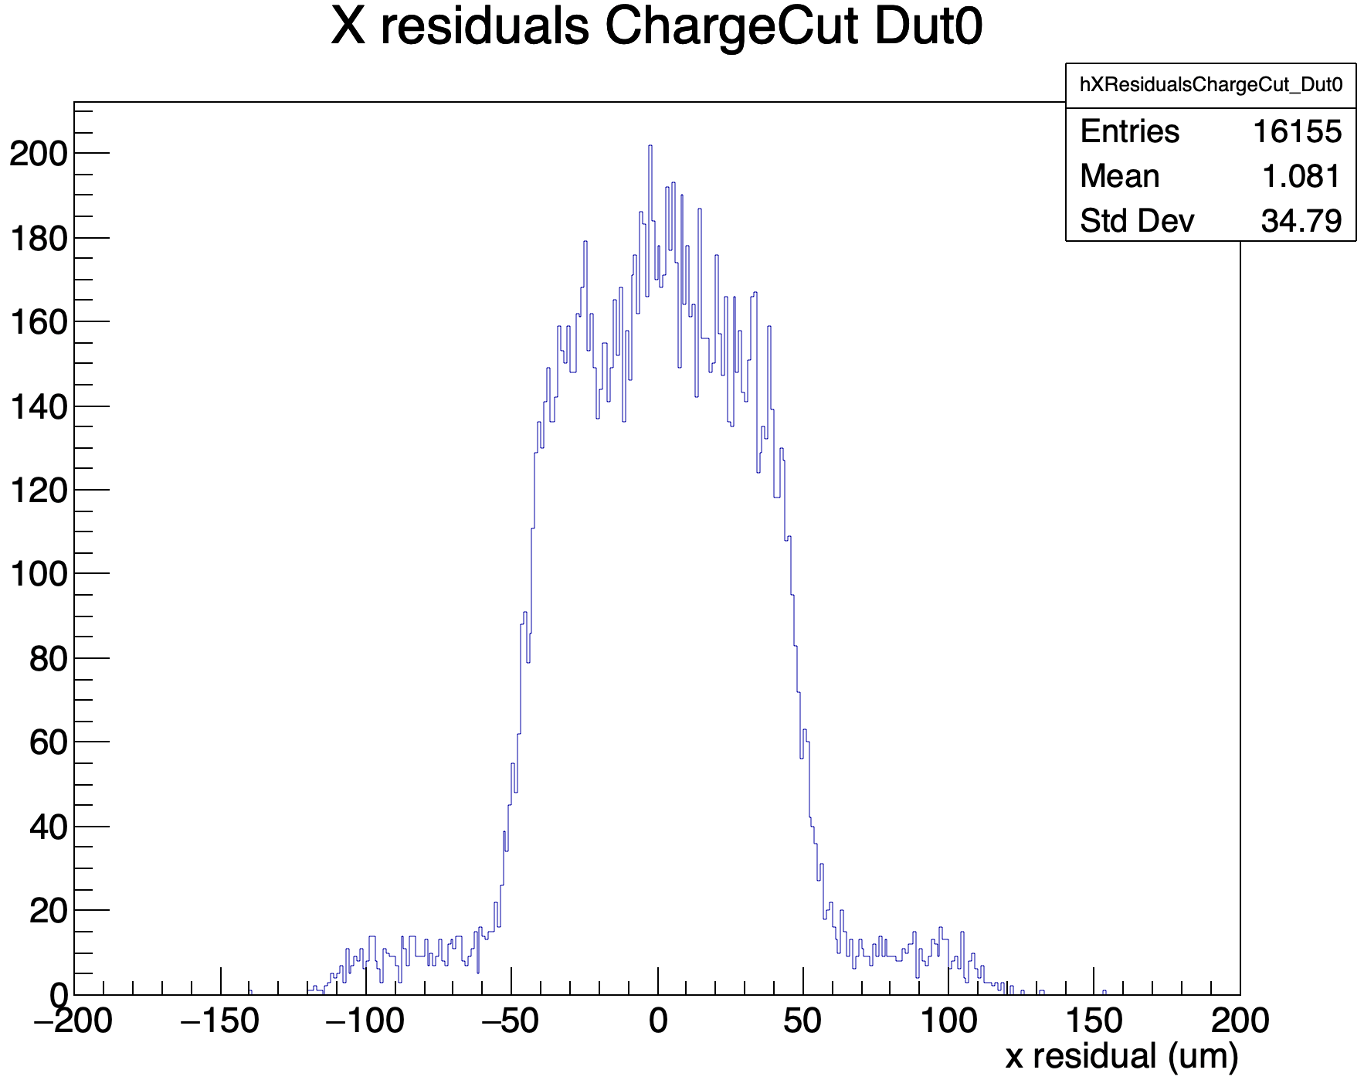
\includegraphics[width=\textwidth]{images/XRes_NoBin0_4pixel.png}
        \caption{}
    \end{subfigure}

    \vspace{0.5cm} % optional spacing between rows

    \begin{subfigure}[b]{0.3\textwidth}
        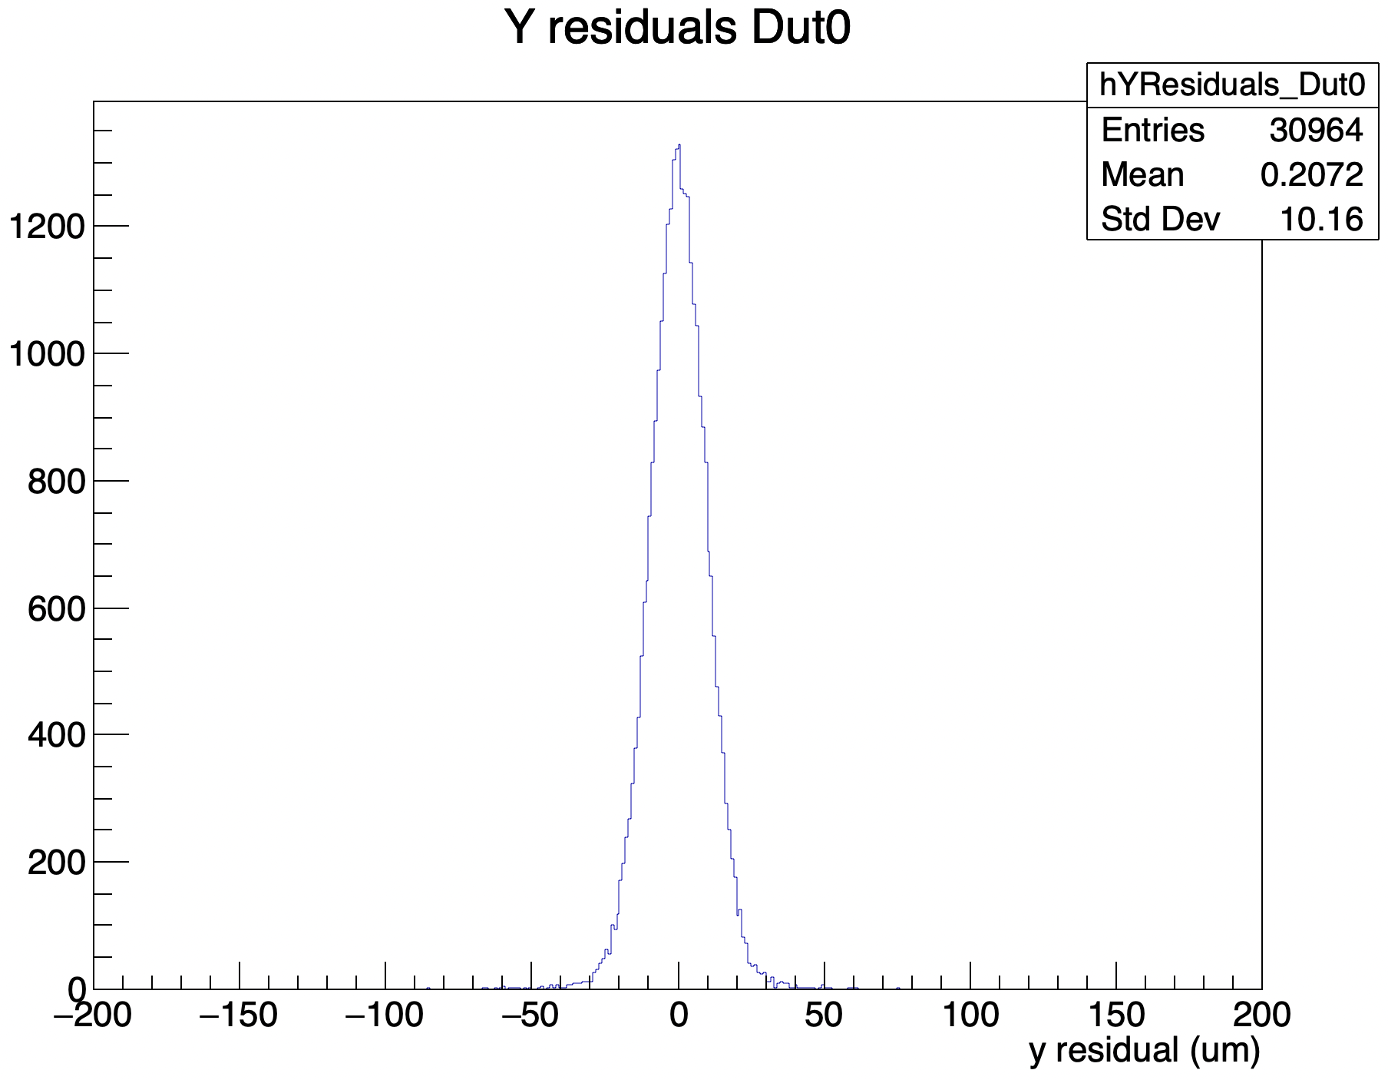
\includegraphics[width=\textwidth]{images/YRes_13planes.png}
        \caption{}
    \end{subfigure}
    \hfill
    \begin{subfigure}[b]{0.33\textwidth}
        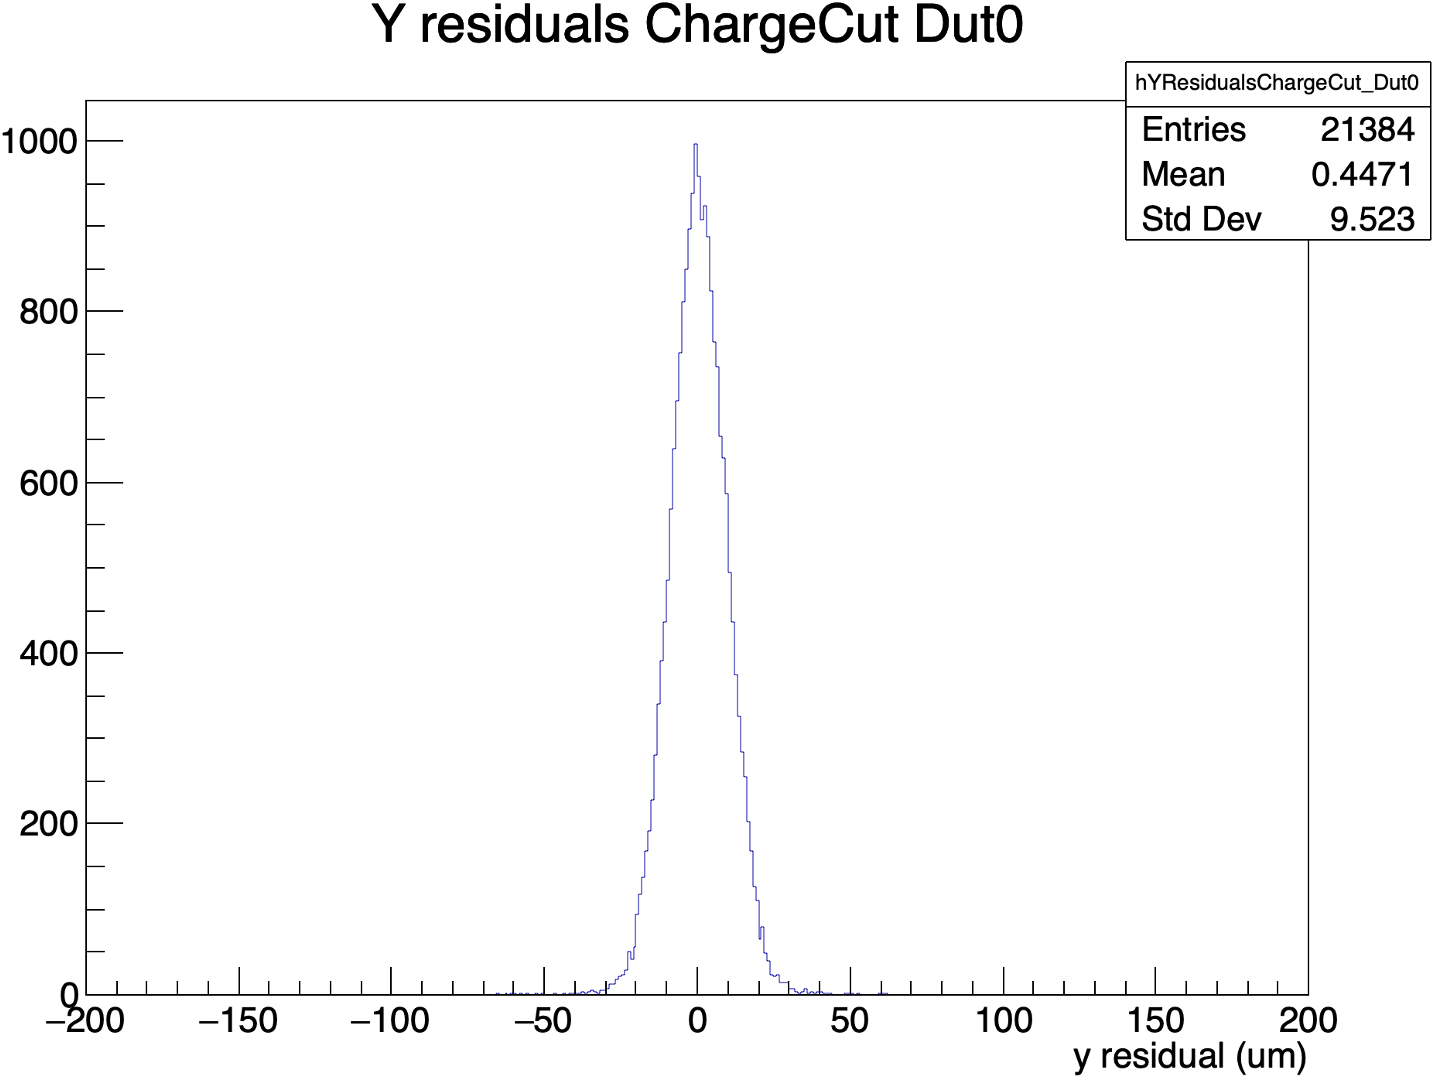
\includegraphics[width=\textwidth]{images/YRes_4pixel.png}
        \caption{}
    \end{subfigure}
    \hfill
    \begin{subfigure}[b]{0.3\textwidth}
        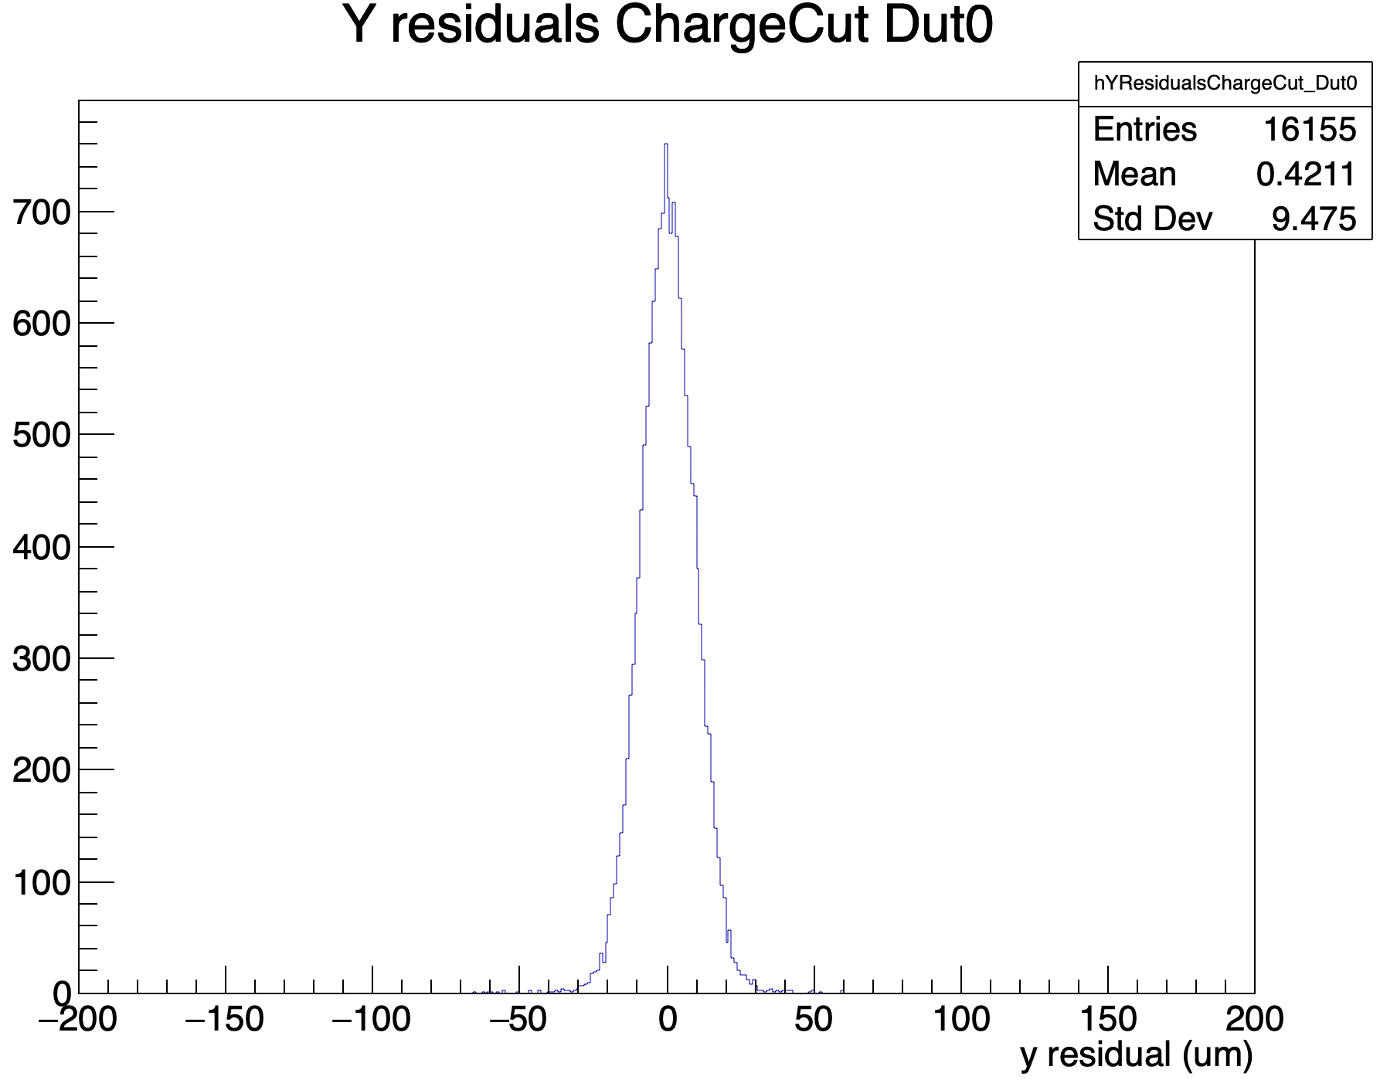
\includegraphics[width=\textwidth]{images/YRes_noBin0_4pixel.png}
        \caption{}
    \end{subfigure}

    \caption{X residuals are shown in panels (a--c): (a) for tracks passing through at least 13 planes, (b) for tracks passing through all 4 pixel planes, and (c) same as (b) but excluding Bin 0 (delta-ray) tracks. Panels (d--f) show the corresponding Y residuals under the same conditions.}
    \label{fig:X_Y_Residual_planes}
\end{figure}

In addition, asymmetry plots for different charge Bins were studied, with the expectation that the delta-ray charge Bin 0 would be more asymmetric than the others, indicating higher crosstalk. The charge asymmetry is defined as \( \frac{C_L - C_R}{C_L + C_R} \), where \( C_L \) and \( C_R \) are the charges collected by the cells to the left and right of the divide, respectively.
The results only for Right bump-bump are shown in Figure~\ref{fig:asymmetry_bins}.

\begin{figure}[H]
    \centering

    \begin{subfigure}[b]{0.3\textwidth}
        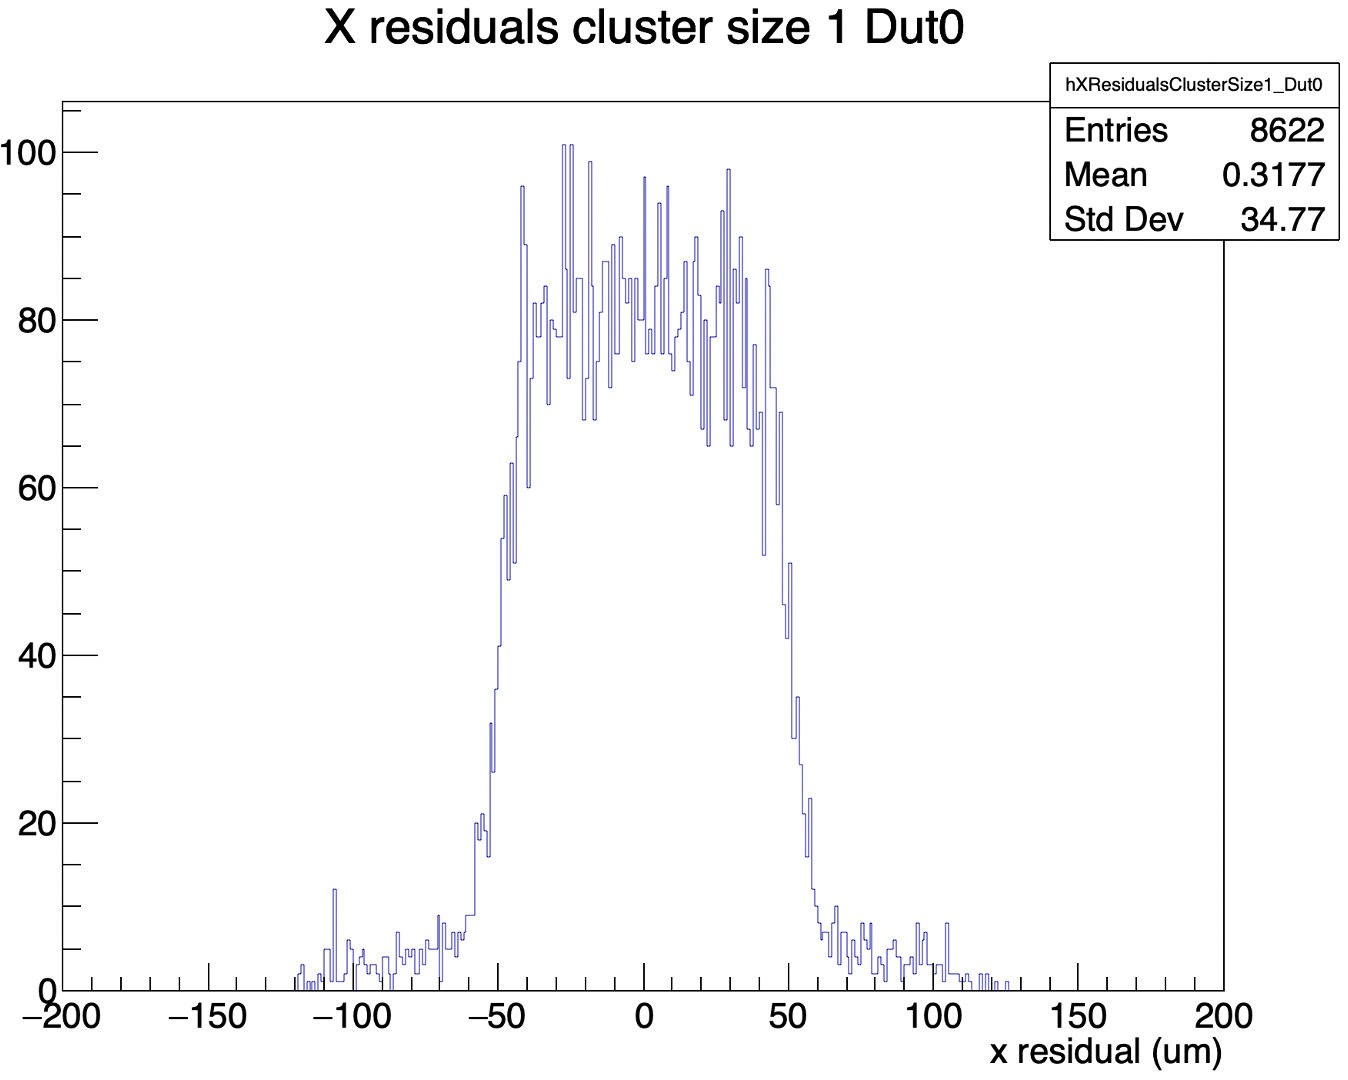
\includegraphics[width=\textwidth]{images/XRes_13plane_size1.png}
        \caption{}
    \end{subfigure}
    \hfill
    \begin{subfigure}[b]{0.33\textwidth}
        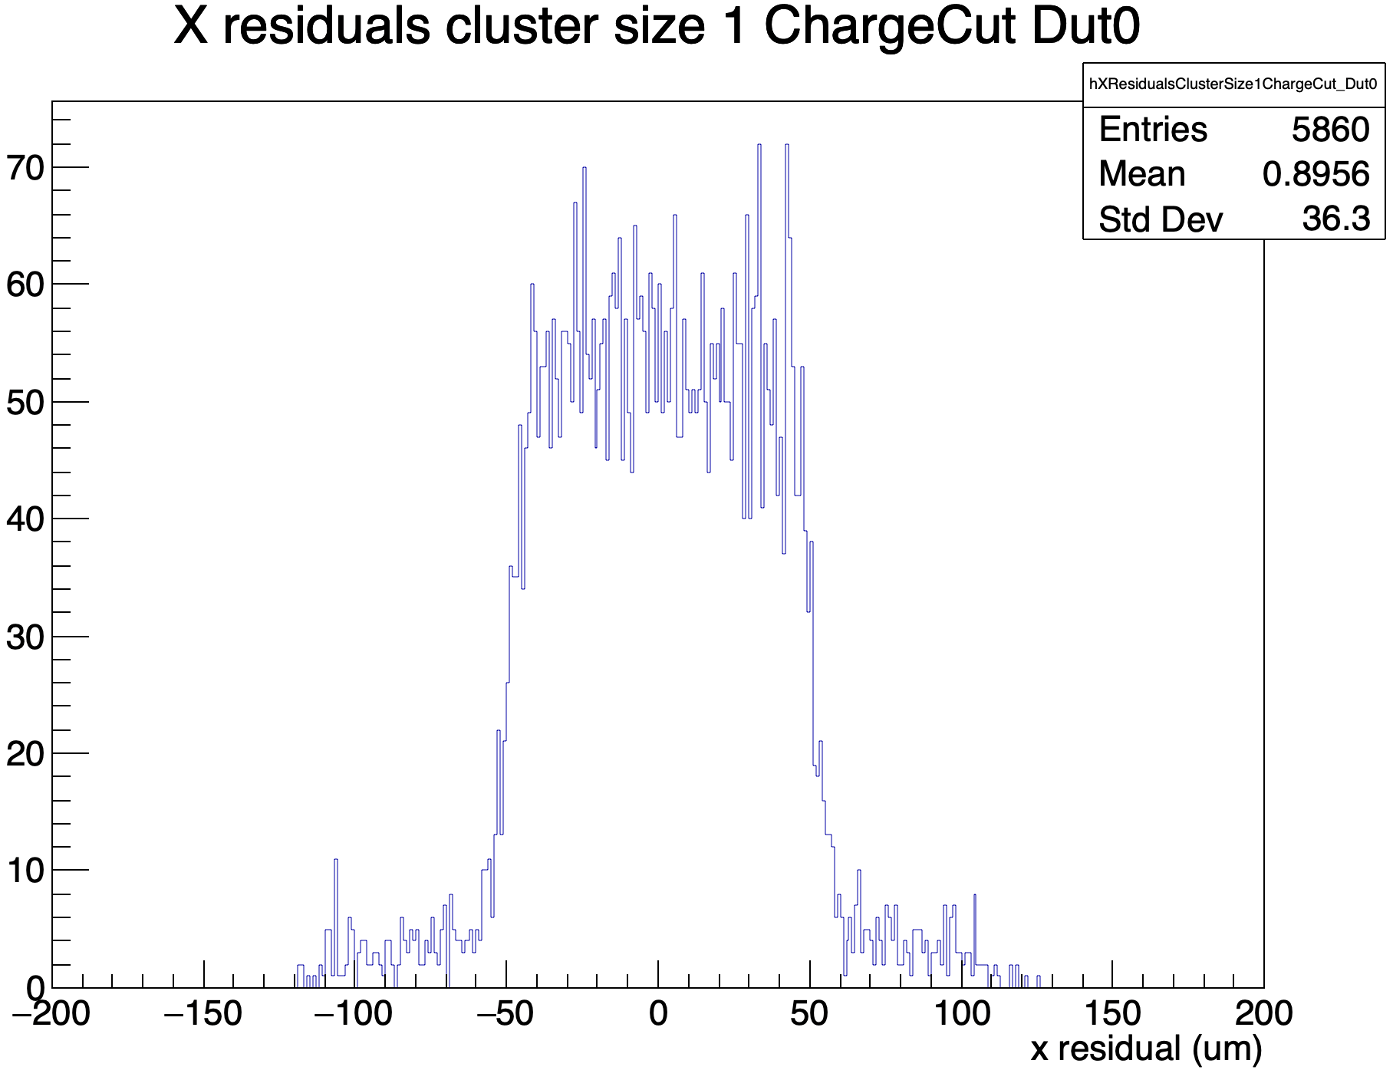
\includegraphics[width=\textwidth]{images/XRes_size1_4pixel.png}
        \caption{}
    \end{subfigure}
    \hfill
    \begin{subfigure}[b]{0.3\textwidth}
        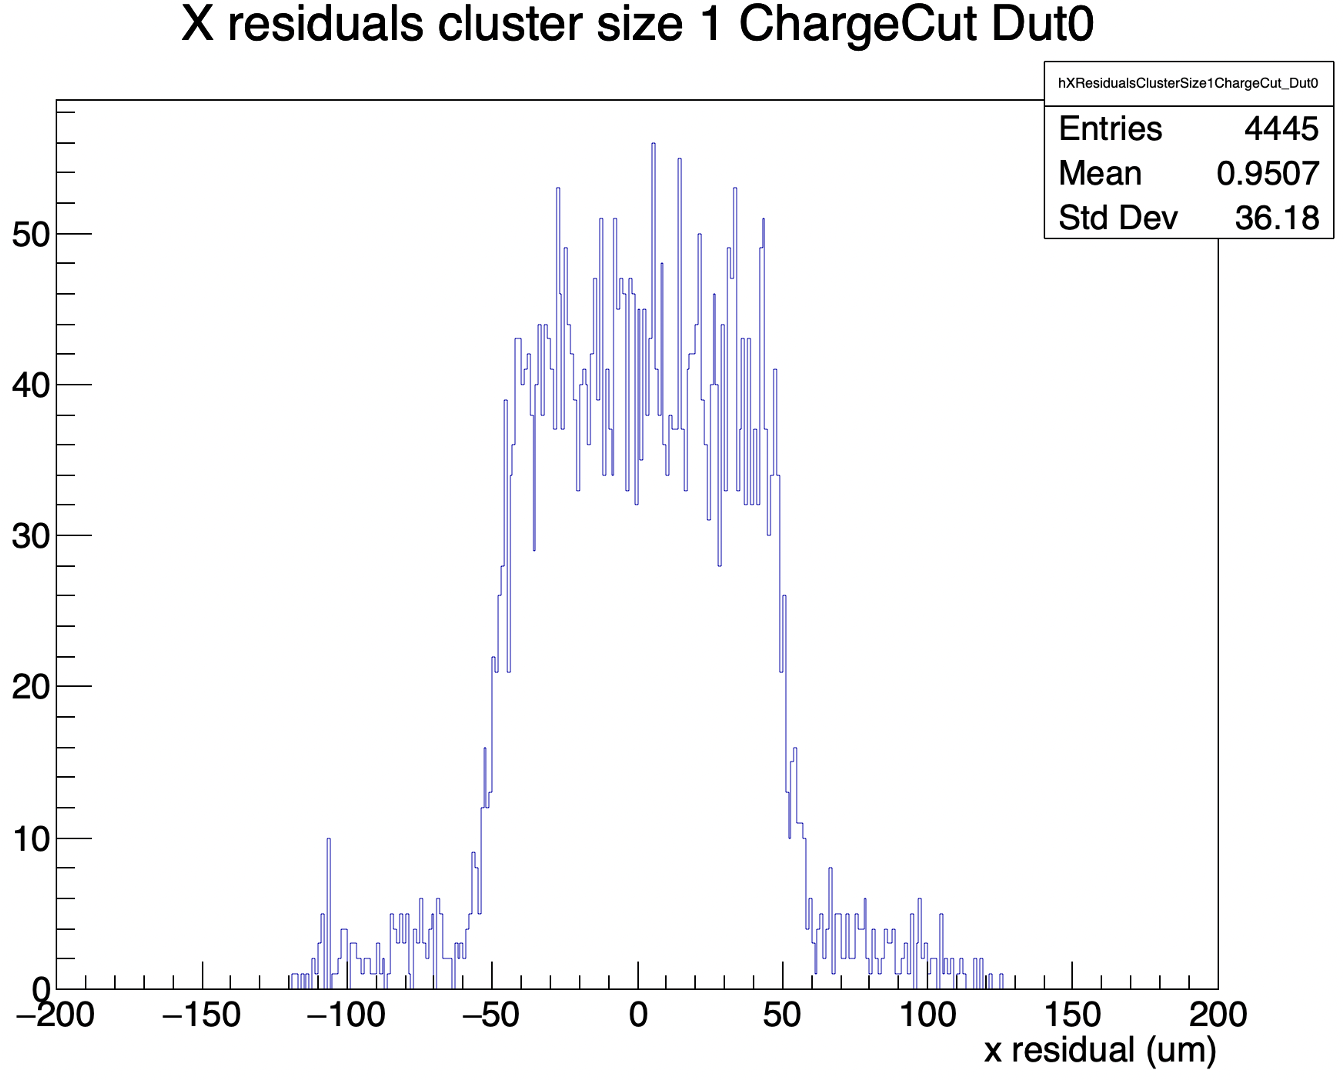
\includegraphics[width=\textwidth]{images/XRes_4pixel_noBin0_size1.png}
        \caption{}
    \end{subfigure}

    \vspace{0.5cm} % optional spacing between rows

    \begin{subfigure}[b]{0.3\textwidth}
        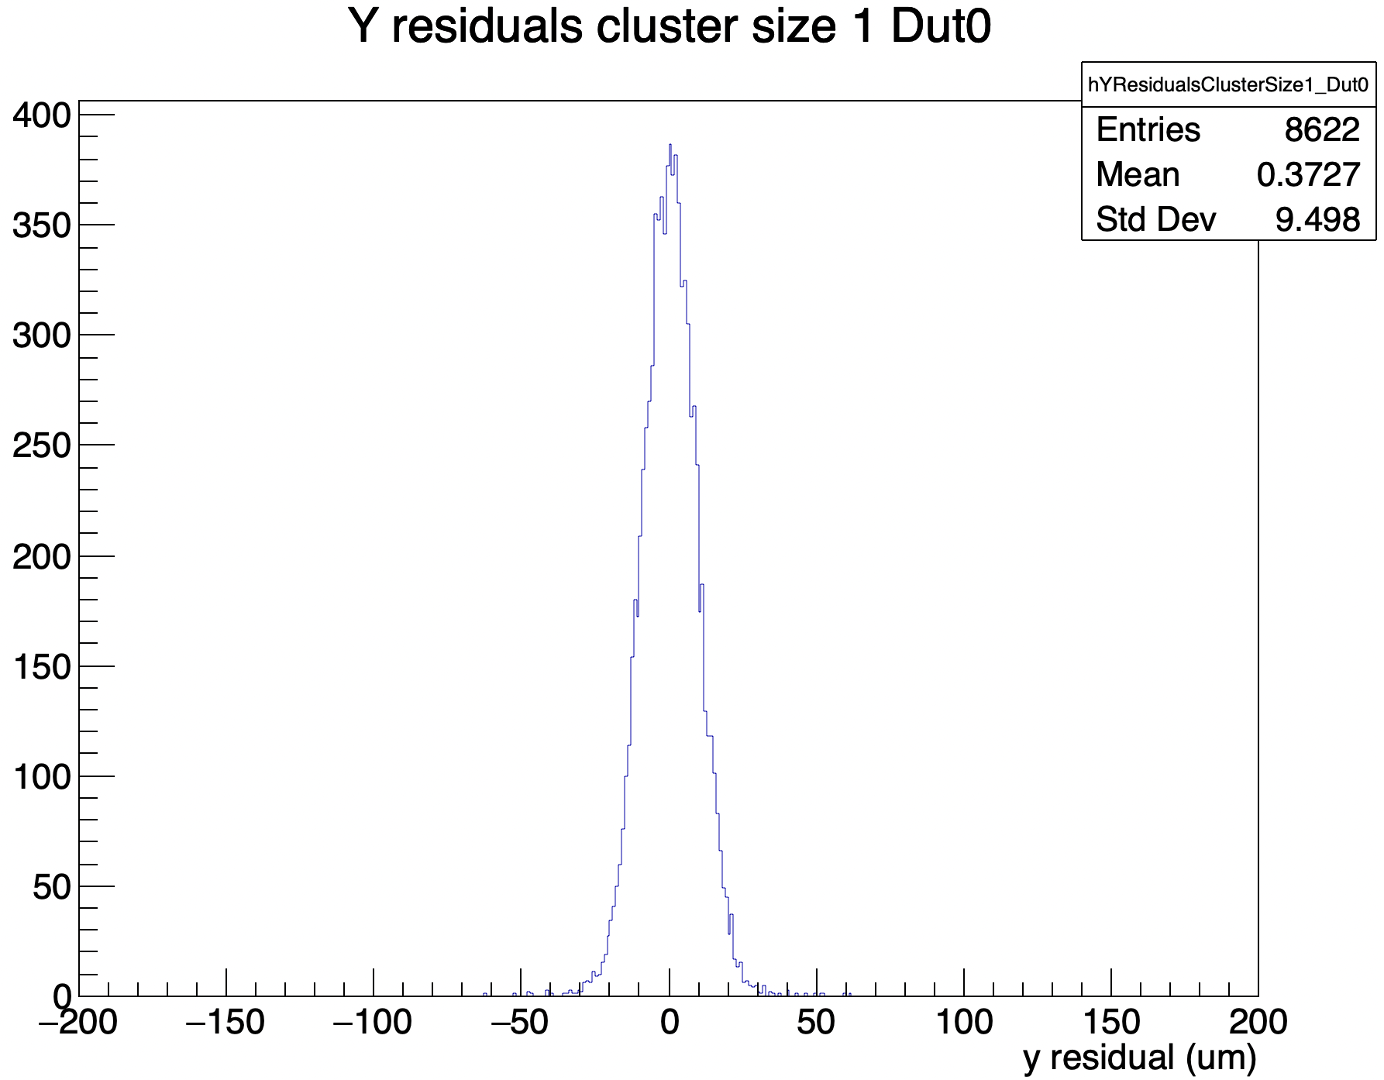
\includegraphics[width=\textwidth]{images/YRes_size1_13planes.png}
        \caption{}
    \end{subfigure}
    \hfill
    \begin{subfigure}[b]{0.33\textwidth}
        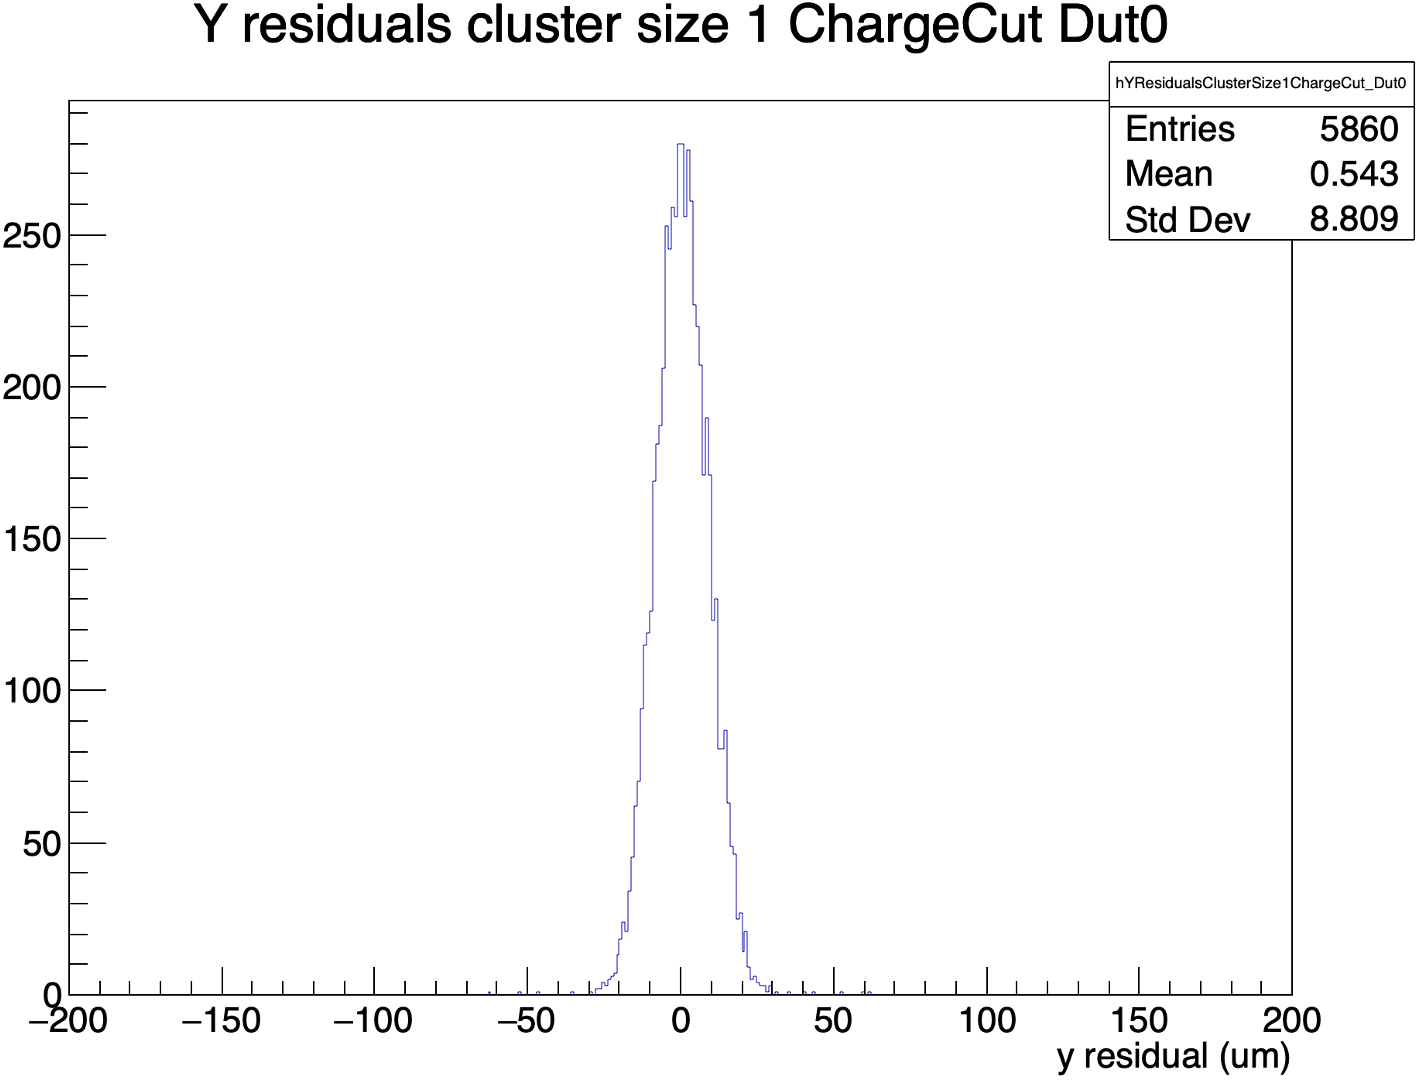
\includegraphics[width=\textwidth]{images/YRes_size1_4pixel.png}
        \caption{}
    \end{subfigure}
    \hfill
    \begin{subfigure}[b]{0.3\textwidth}
        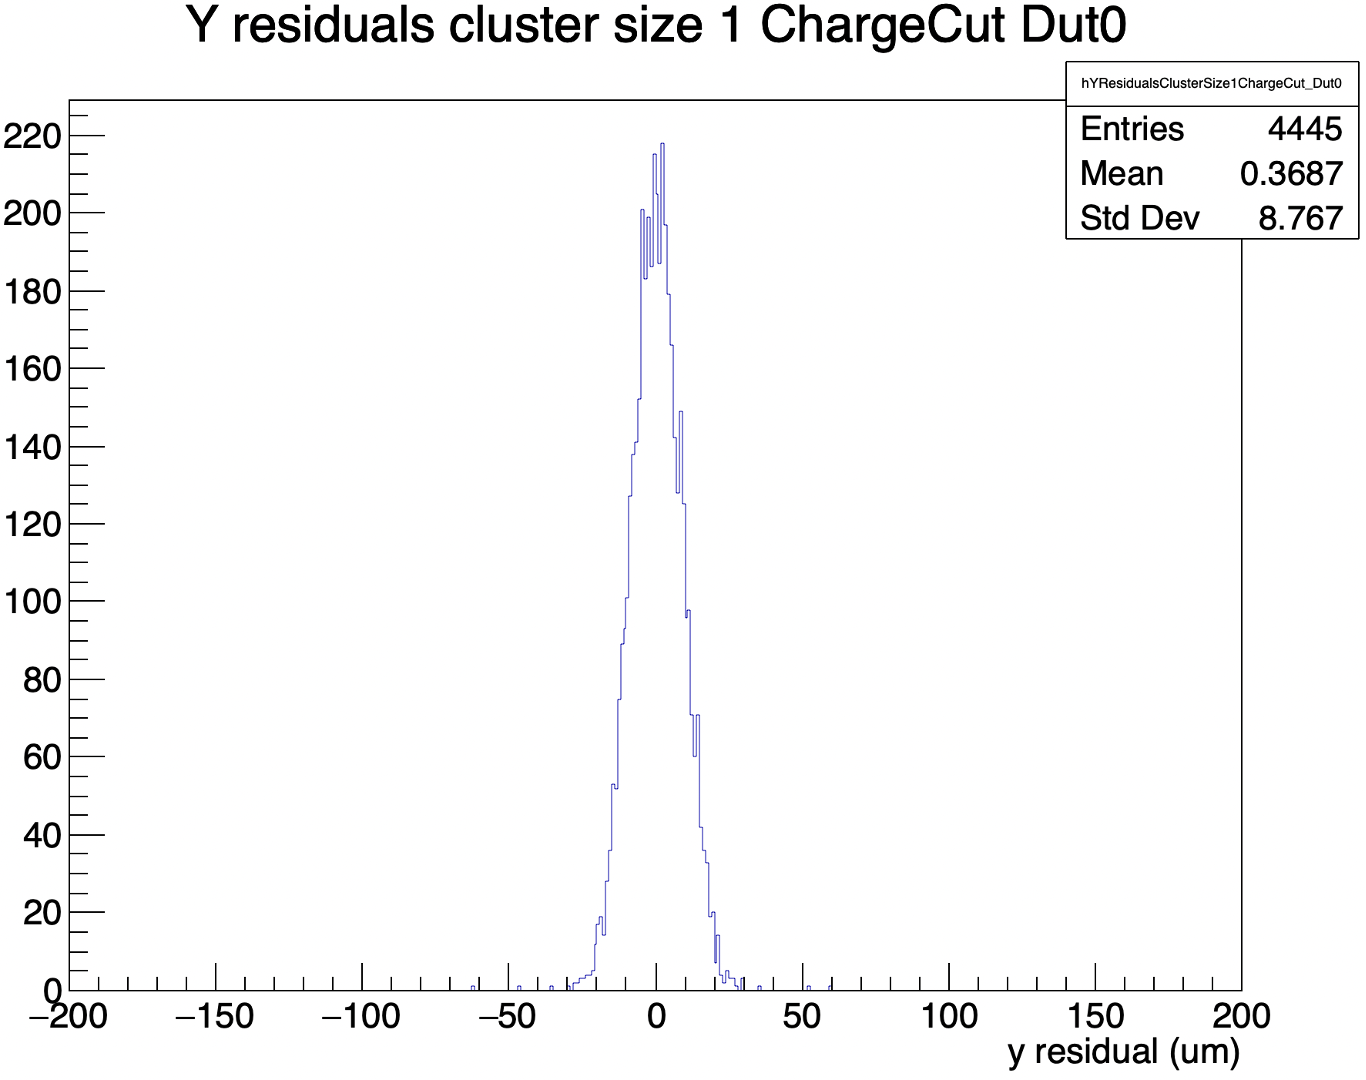
\includegraphics[width=\textwidth]{images/YRes_size1_4pixel_noBin0.png}
        \caption{}
    \end{subfigure}

    \caption{X residuals for cluster size 1 shown in (a--c): (a) using tracks that pass through at least 13 planes, (b) requiring tracks to pass through all 4 pixel planes, and (c) same as (b) but with Bin 0 (delta-ray) tracks excluded. Panels (d--f) show the corresponding Y residuals under the same conditions.}
    \label{fig:X_Y_Residual_size_1_planes}
\end{figure}

In addition, asymmetry plots for different charge Bins were studied, with the expectation that the delta-ray charge Bin~0 would be more asymmetric than the others, indicating higher crosstalk. The charge asymmetry is defined as
\[
\text{Asymmetry} = \frac{C_L - C_R}{C_L + C_R},
\]
where \( C_L \) and \( C_R \) are the charges collected by the cells to the left and right of the divide, respectively. The results for the right bump-bonded side are shown in Figure~\ref{fig:asymmetry_bins}. However, it is difficult to interpret the results for charge Bin~0 due to the relatively small number of entries compared to the other Bins. Furthermore, it was observed that data points near the asymmetry values of 1 and $-1$ mostly correspond to charge-shared clusters. Despite this, a clear interpretation is still challenging, as no quantitative measure of the asymmetry has been established so far. Therefore, further investigation is needed for better understanding of this behavior.

\begin{figure}[H]
    \centering
    \begin{subfigure}[t]{0.45\textwidth}
        \centering
        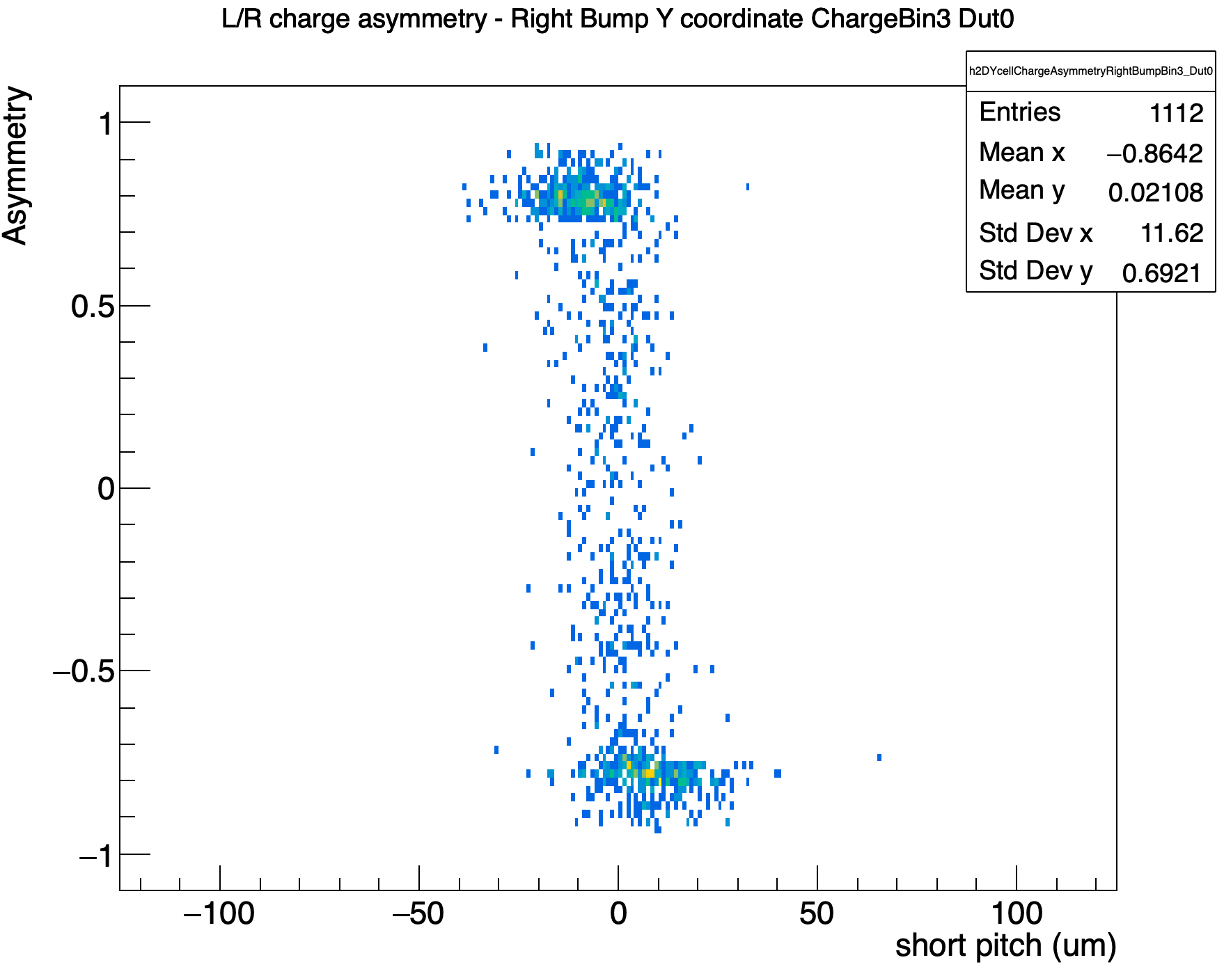
\includegraphics[width=\textwidth]{images/YAsymBin3.png}
        \caption{}
        \label{fig:dist_a}
    \end{subfigure}
    \hfill
    \begin{subfigure}[t]{0.45\textwidth}
        \centering
        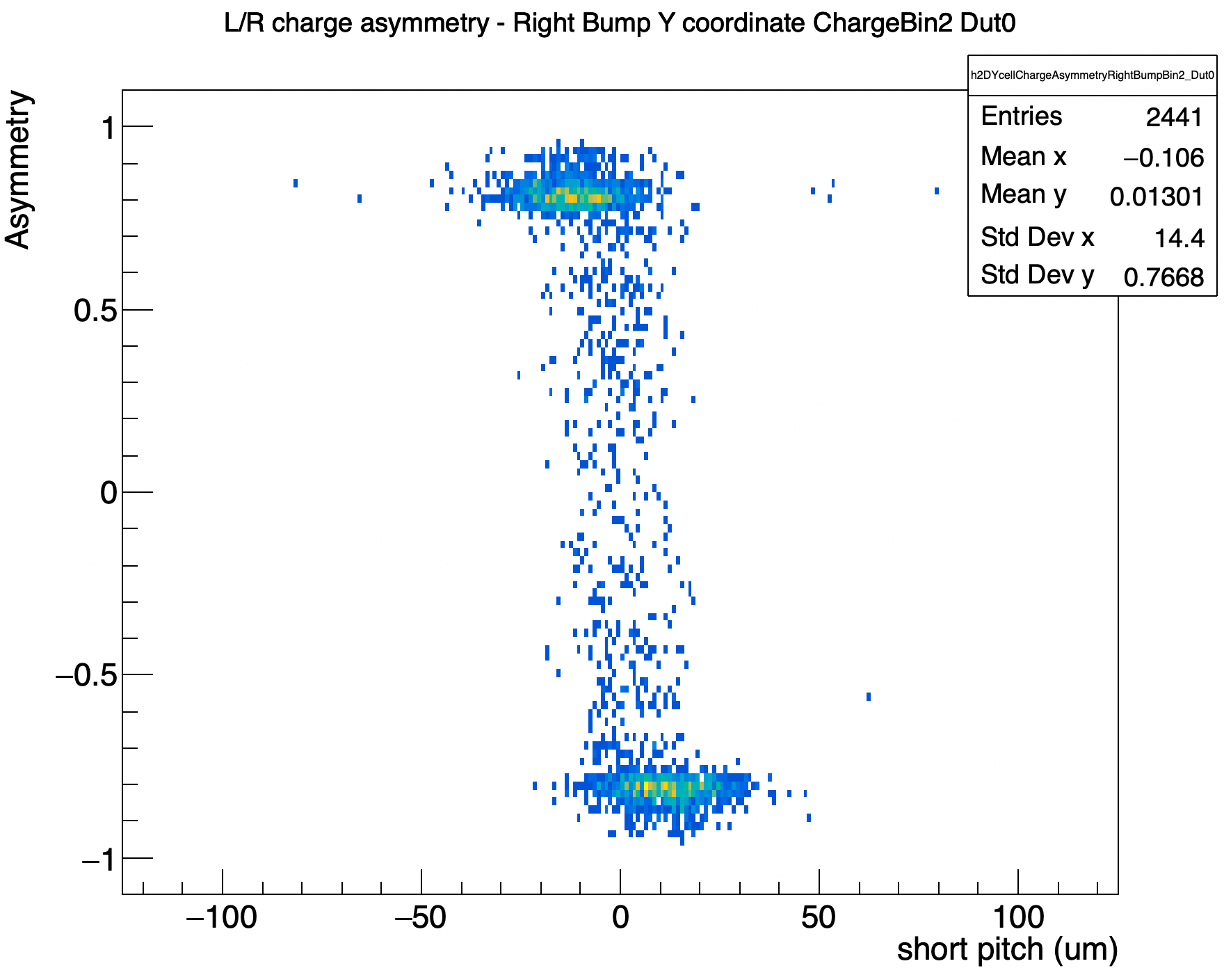
\includegraphics[width=\textwidth]{images/YAsymBin2.png}
        \caption{}
        \label{fig:dist_b}
    \end{subfigure}

    \vspace{0.5cm}

    \begin{subfigure}[t]{0.45\textwidth}
        \centering
        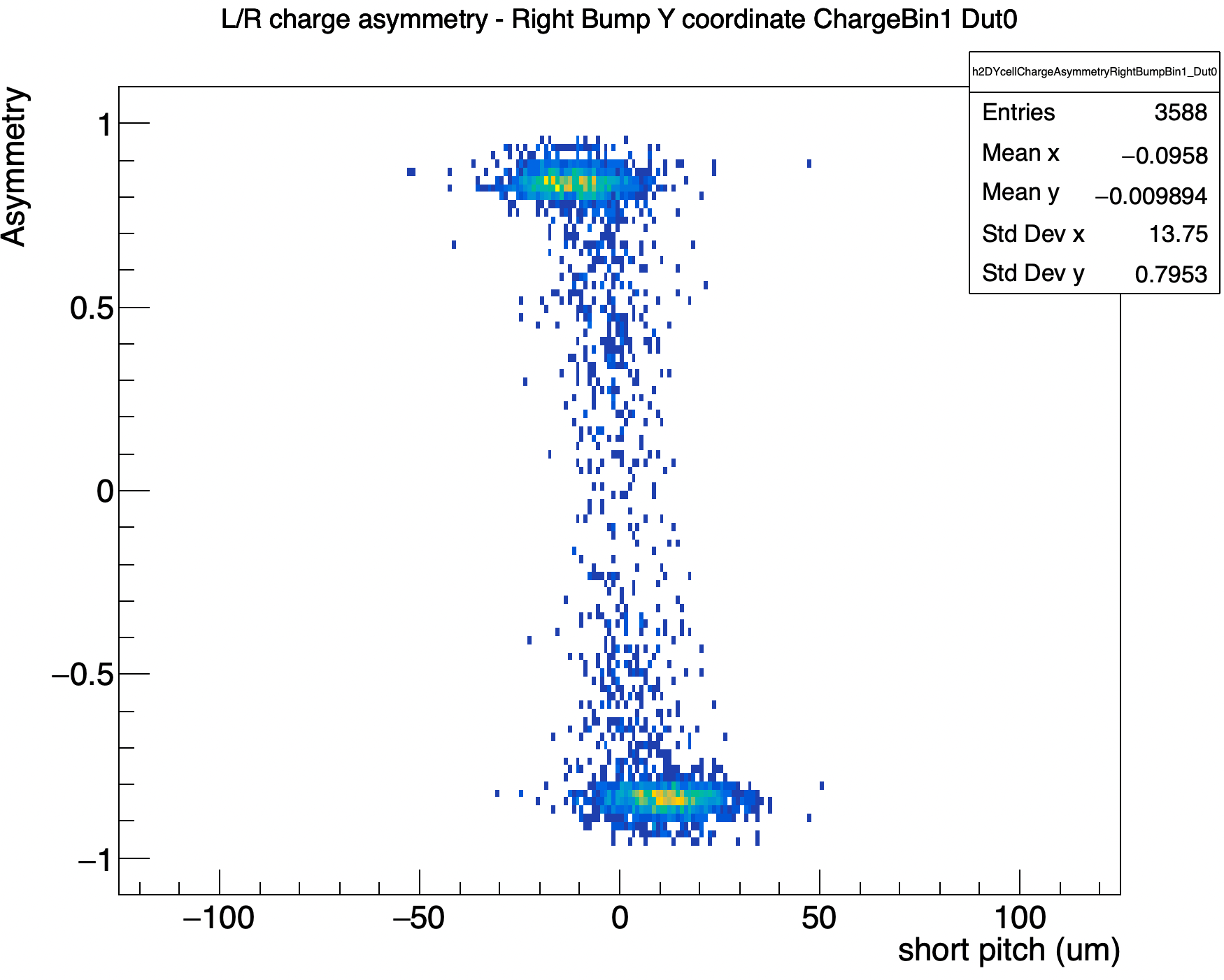
\includegraphics[width=\textwidth]{images/YAsymmetryRightBin1.png}
        \caption{}
        \label{fig:dist_c}
    \end{subfigure}
    \hfill
    \begin{subfigure}[t]{0.45\textwidth}
        \centering
        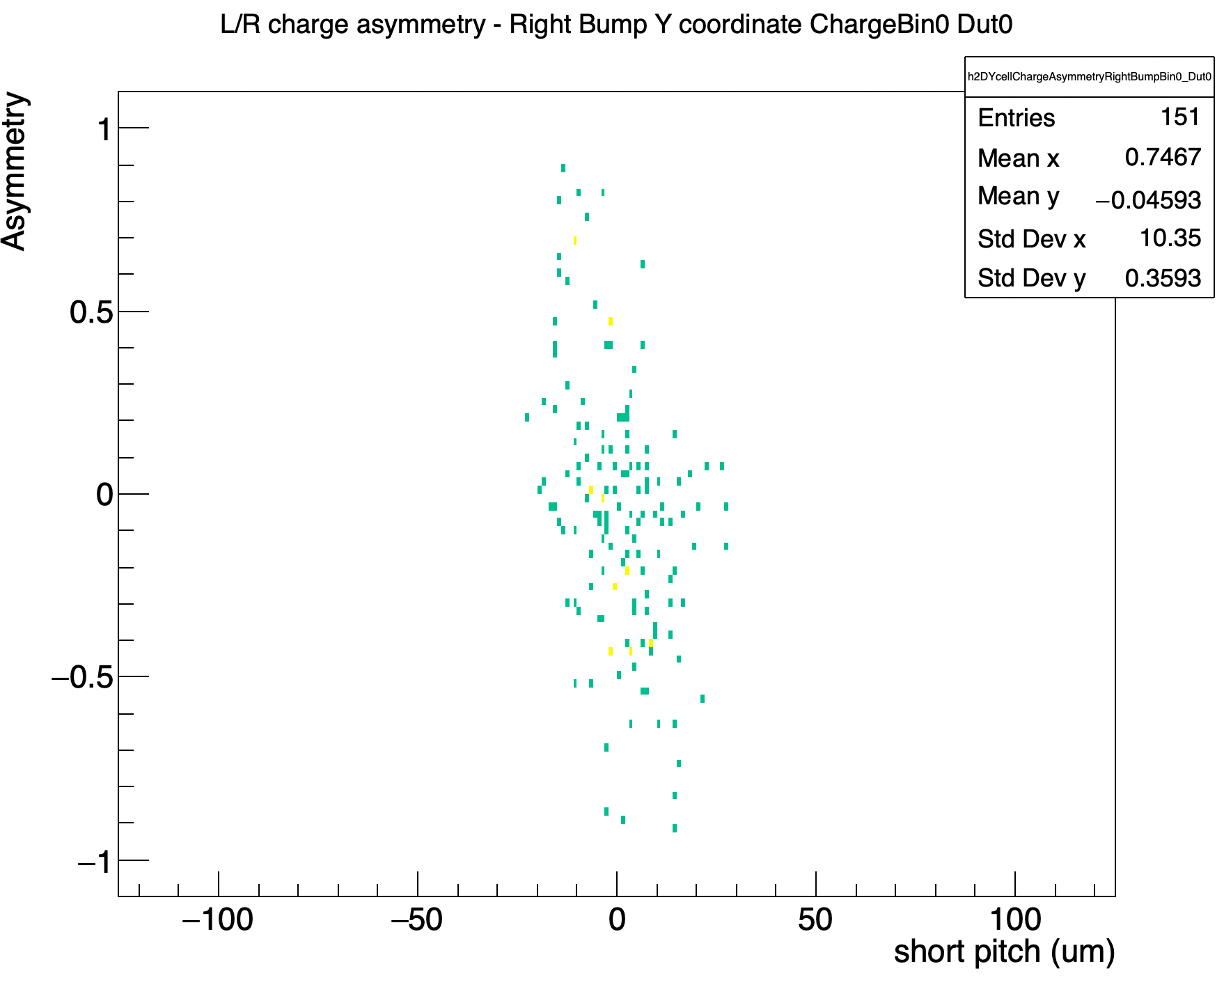
\includegraphics[width=\textwidth]{images/YAsymmetryRightBumpBin0.png}
        \caption{}
        \label{fig:dist_d}
    \end{subfigure}

    \caption{Asymmetry plot for all of the charge Bins.}
    \label{fig:asymmetry_bins}
\end{figure}

\subsection{NMF for 1D Data Quality Monitoring}

Typically, input data are represented by a particular ME (1D so far) for each LS of the RR, and after some minor filtering, the model is trained on it. Test or target data have the training data as a reference used for certification. After some prefiltering based on the basis matrix, the coefficient matrix for the test data may be found. However, in order to identify actual anomalies and prove the concept of the model, fake test data were produced such that the first LS corresponds to an actual LS from the training data. In particular, in this case, the charge distribution for Pixel Layer 1 was observed. The remaining LSs were generated by shifting the peak of the Landau-like distribution to the left, bin by bin. The total number of generated fake data LSs is 14 see Figure~\ref{fig:fake_data}.

\begin{figure}[H]
    \centering
    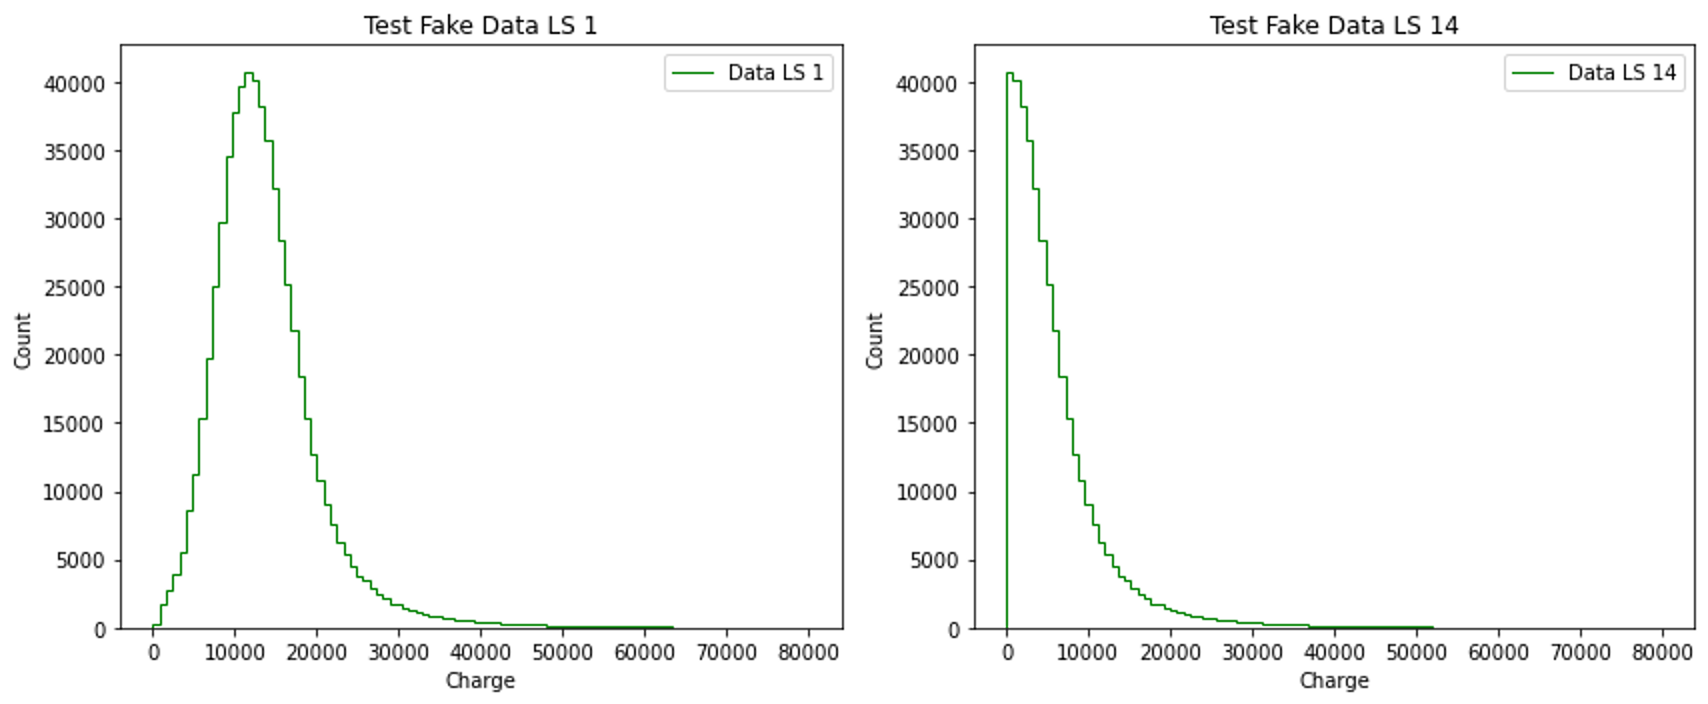
\includegraphics[width=0.9\textwidth]{images/fake_input.png}
    \caption{Fake data generated (first and last LSs) for the NMF model. The first LS corresponds to the actual data, while the remaining LSs are shifted by one bin to the left.}
    \label{fig:fake_data}
\end{figure}

The model was trained on one of the RRs. The optimal number of components for this case is 4. The basis components are shown in Figure~\ref{fig:components}. It is clearly noticeable that the first component is dominant and represents the main trend of the data (not normalized). The other components are shifted distributions. These components reconstruct the target fake data with different weights assigned to each of them.

\begin{figure}[H]
    \centering
    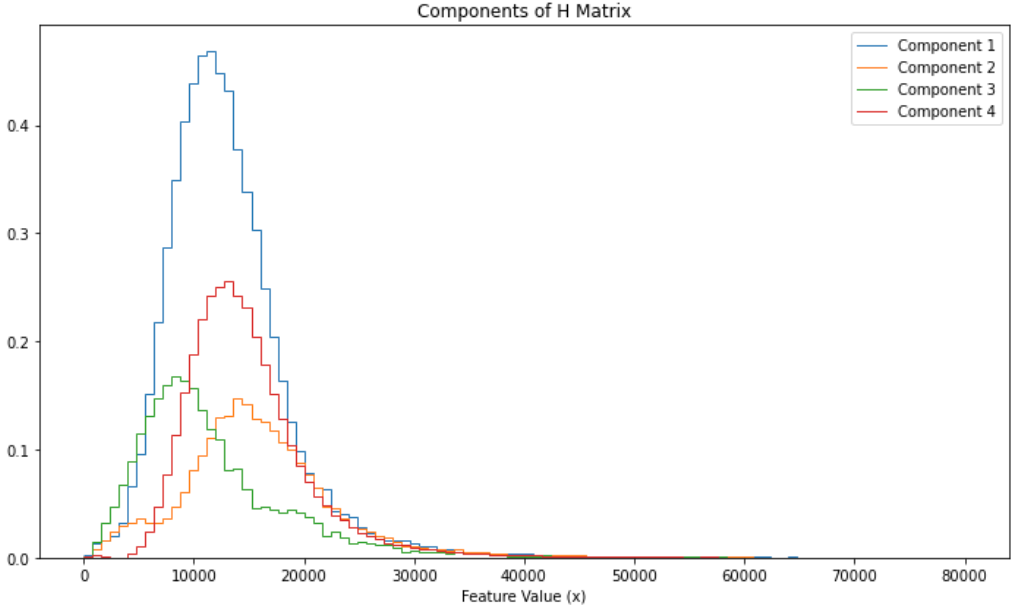
\includegraphics[width=0.8\textwidth]{images/Hcomponents.png}
    \caption{Basis components out of the \( H \) matrix.}
    \label{fig:components}
\end{figure}

\begin{figure}[H]
    \centering
    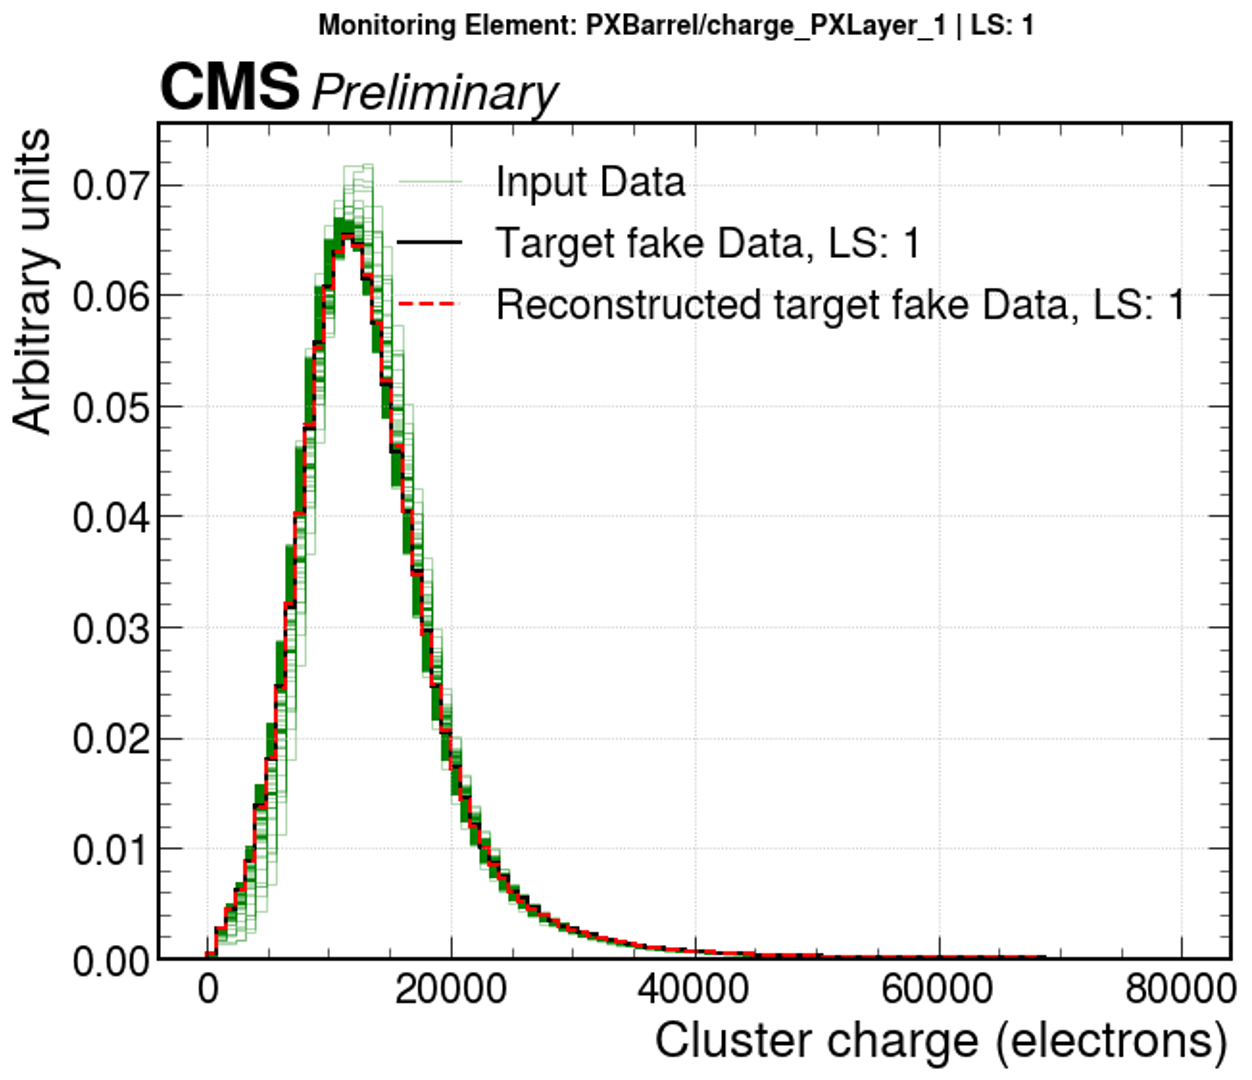
\includegraphics[width=0.48\textwidth]{images/fake_reco_ls1.png}
    \hfill
    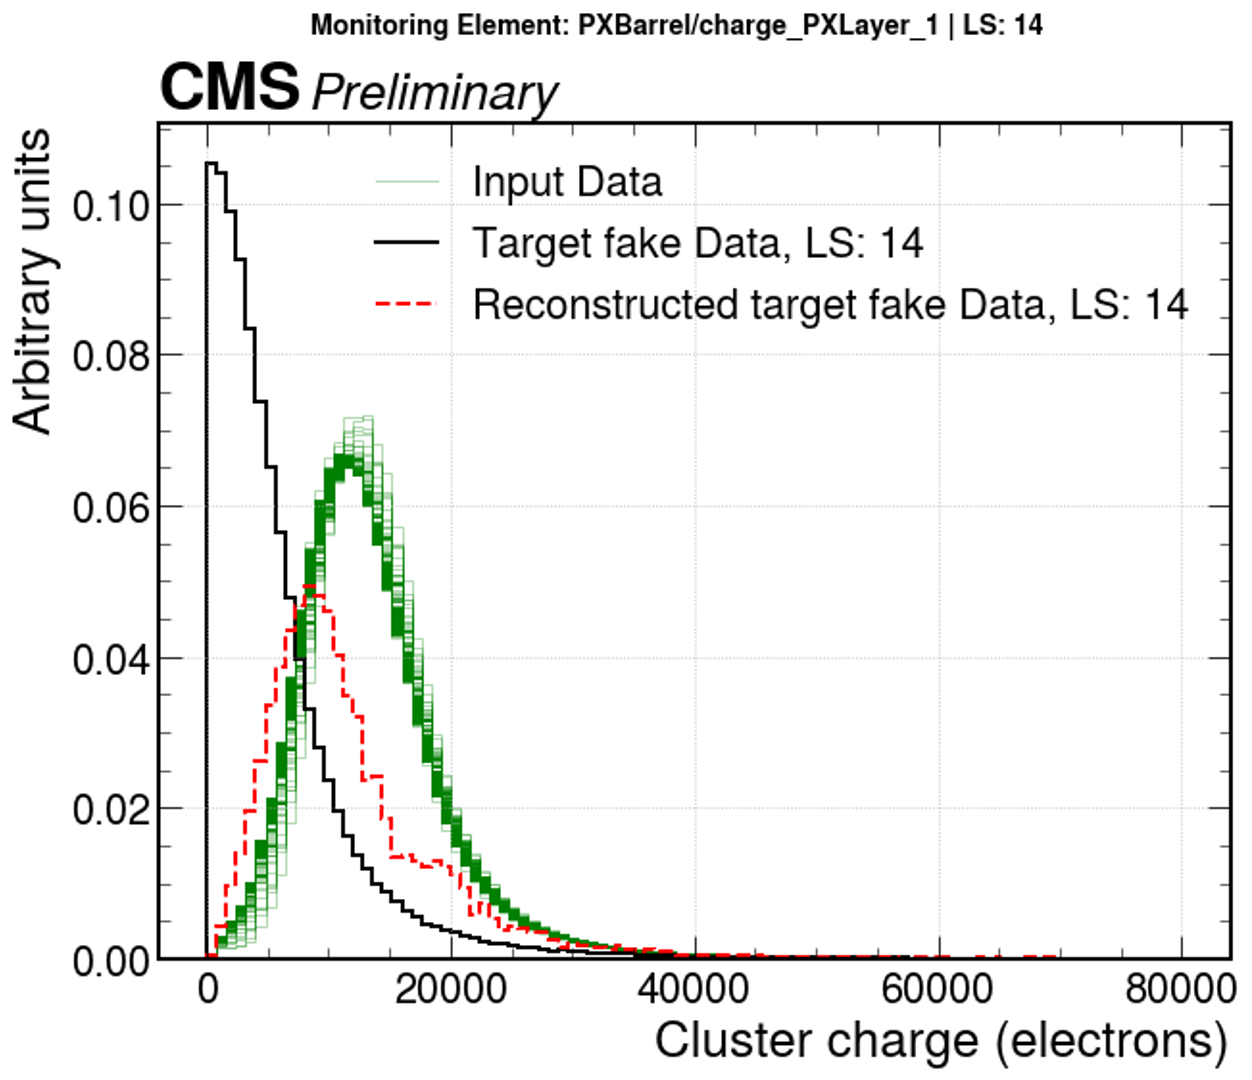
\includegraphics[width=0.48\textwidth]{images/fake_reco_ls14.png}
    \caption{Reconstruction of the 1st (left) and 14th (right) LSs from the fake dataset. The red lines show the model’s reconstruction of fake data, while the green lines represent the overlaid histograms from all training LSs, serving as a reference.}
    \label{fig:reconstruction}
\end{figure}

The reconstruction of these two LSs of the fake data is shown in Figure~\ref{fig:reconstruction}. The label "Input data" corresponds to the training data and is shown in the figures in green. These green histograms represent all of the training data LSs overlaid in order to compare the shifts of the training data with the target fake data. Since the first LS corresponds to actual, true data, its reconstruction looks good and is represented by a noticeable red histogram. Red reconstruction histogram for the first LS overlap with the green ones. However, for the last LS which has the maximum shift in the charge distribution, the reconstruction clearly fails. The red histogram again represents the reconstruction, with the same overlay of training data in green. Therefore, this LS is clearly anomalous. However, in order to apply the model to real data, it is necessary to define a metric to determine the anomaly threshold.

Metrics chosen for identifying anomaly:
\begin{itemize}
    \item Trends for component by the contribution of the area to the distribution see Figure~\ref{fig:trend_plots}
    \item Euclidean distance see Figure~\ref{fig:euc_distance}
    \item Mean squared error (MSE) see Figure~\ref{fig:MSE}
\end{itemize}

\begin{figure}[H]
    \centering
    \begin{subfigure}[t]{1\textwidth}
        \centering
        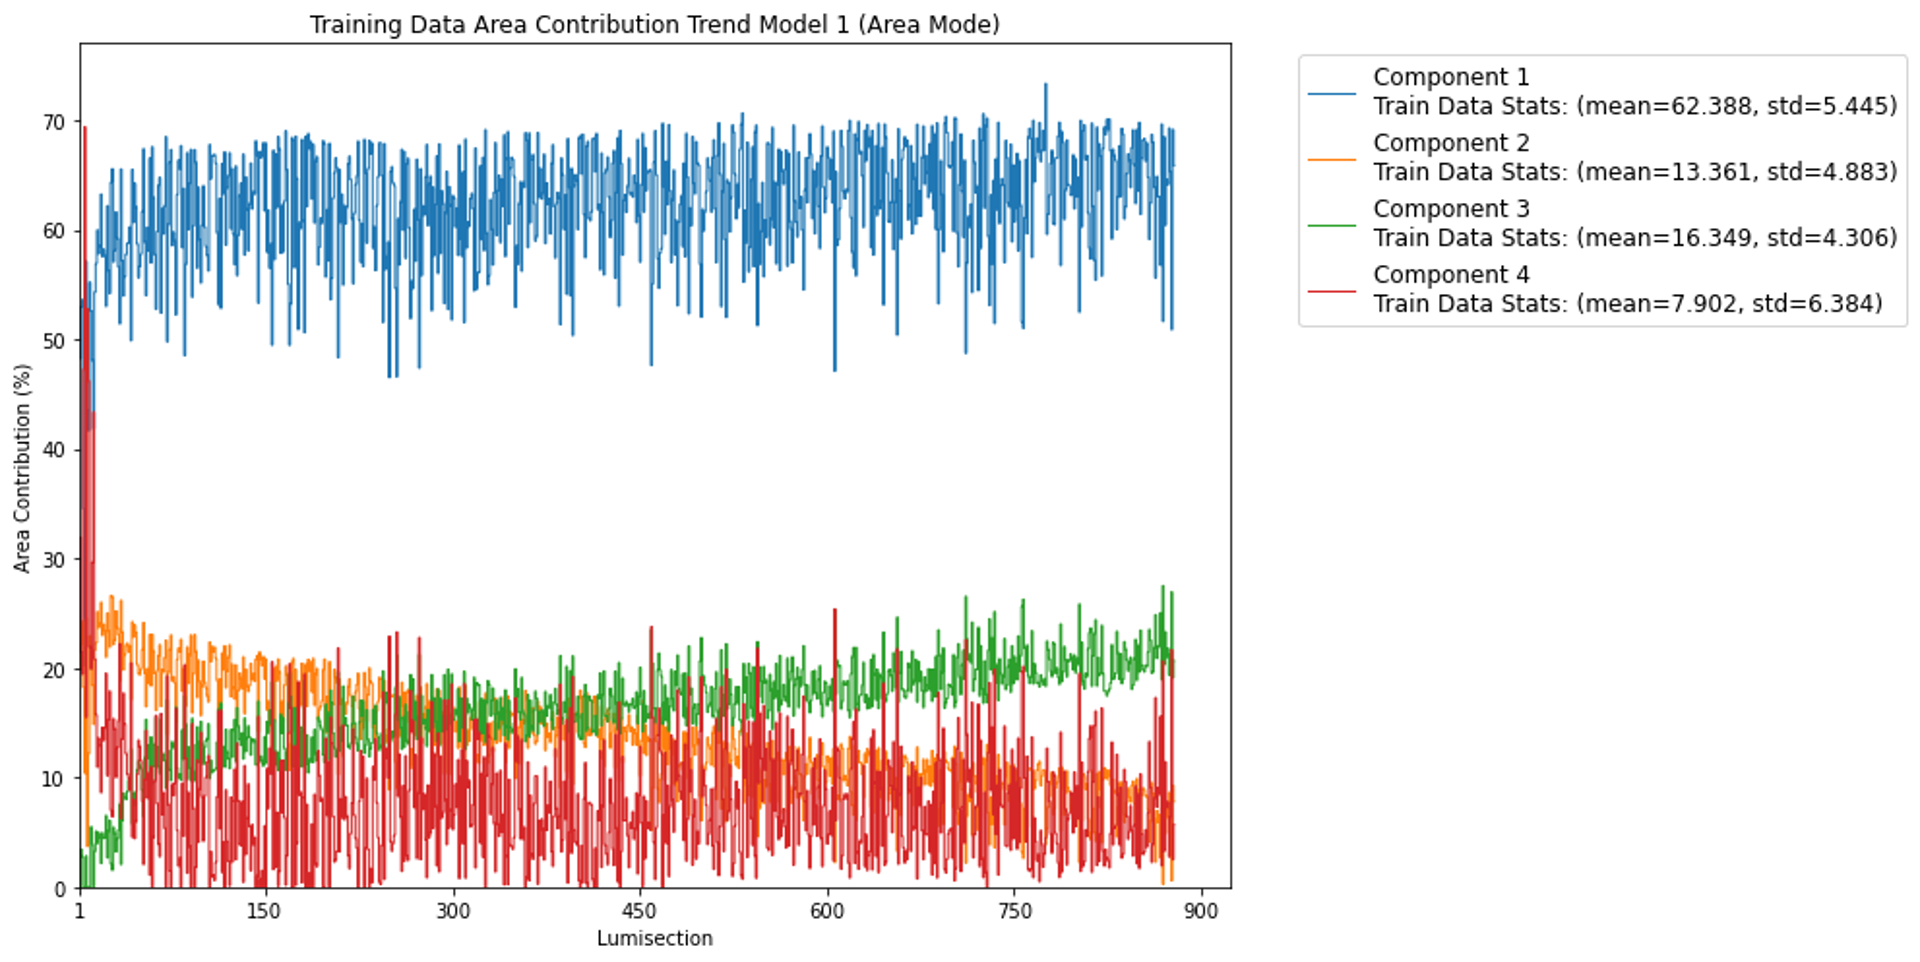
\includegraphics[width=\textwidth]{images/trend_train.png}
    \end{subfigure}
    \hfill
    \begin{subfigure}[t]{1\textwidth}
        \centering
        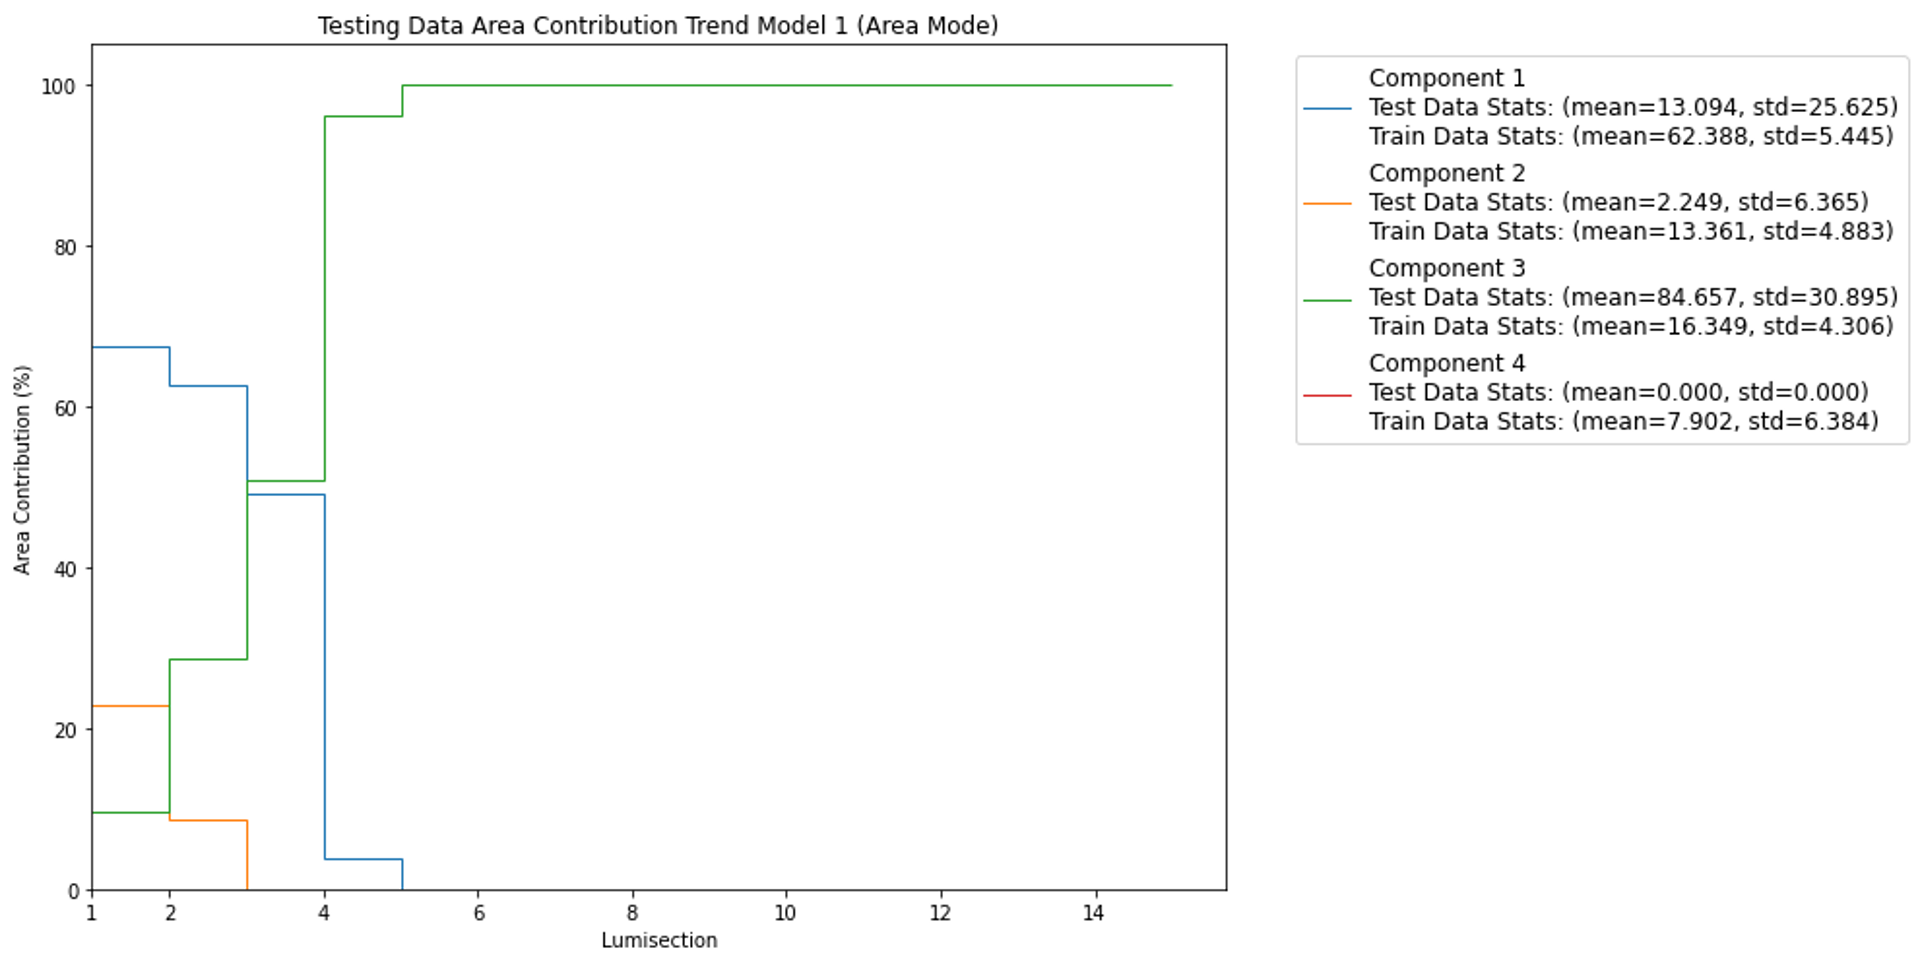
\includegraphics[width=\textwidth]{images/trend_fake.png}
    \end{subfigure}
    \caption{Trend plots.}
    \label{fig:trend_plots}
\end{figure}

\begin{figure}[H]
    \centering
    \begin{subfigure}[t]{1\textwidth}
        \centering
        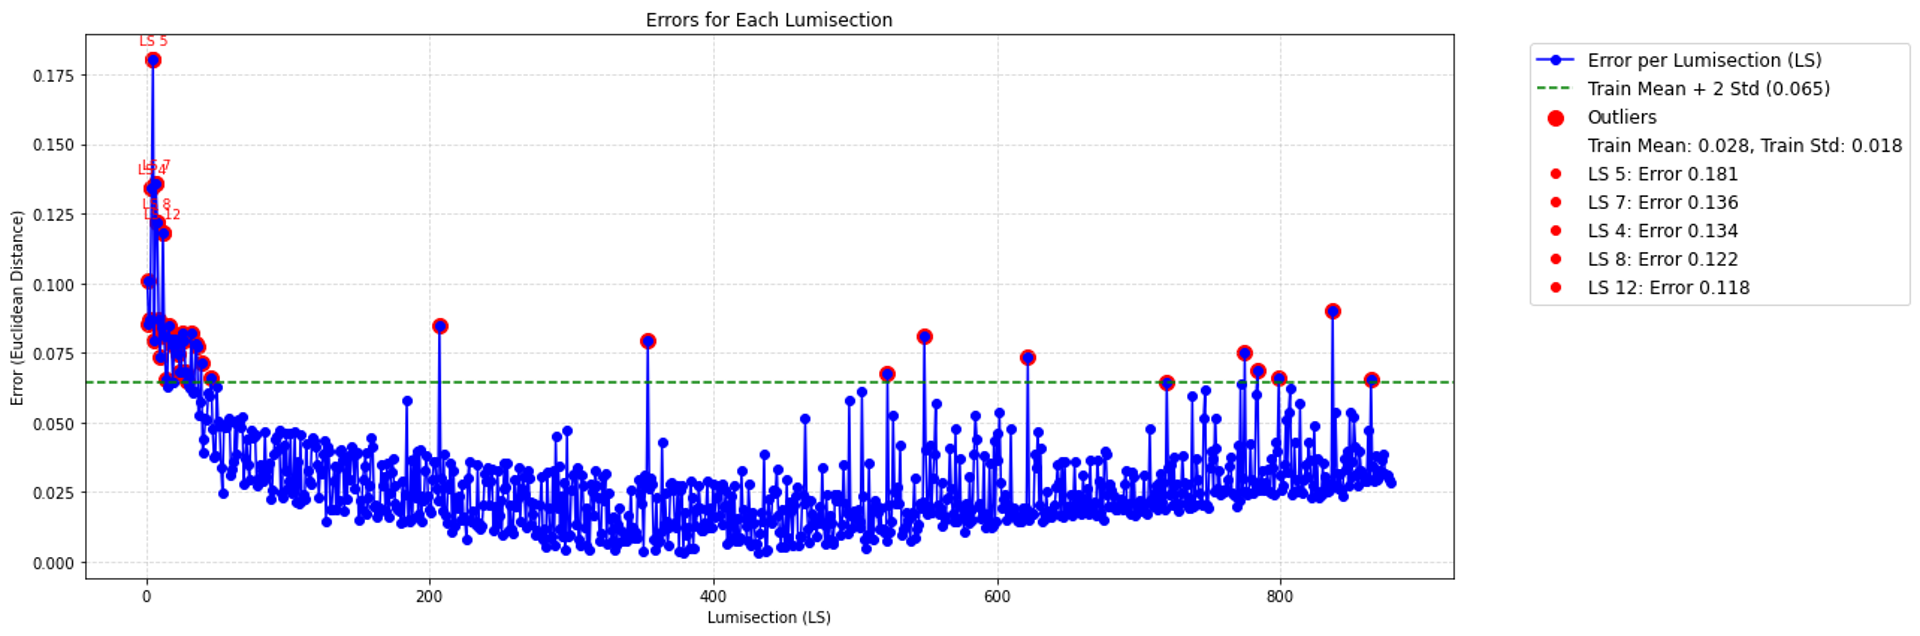
\includegraphics[width=\textwidth]{images/euclid_train.png}
    \end{subfigure}
    \hfill
    \begin{subfigure}[t]{1\textwidth}
        \centering
        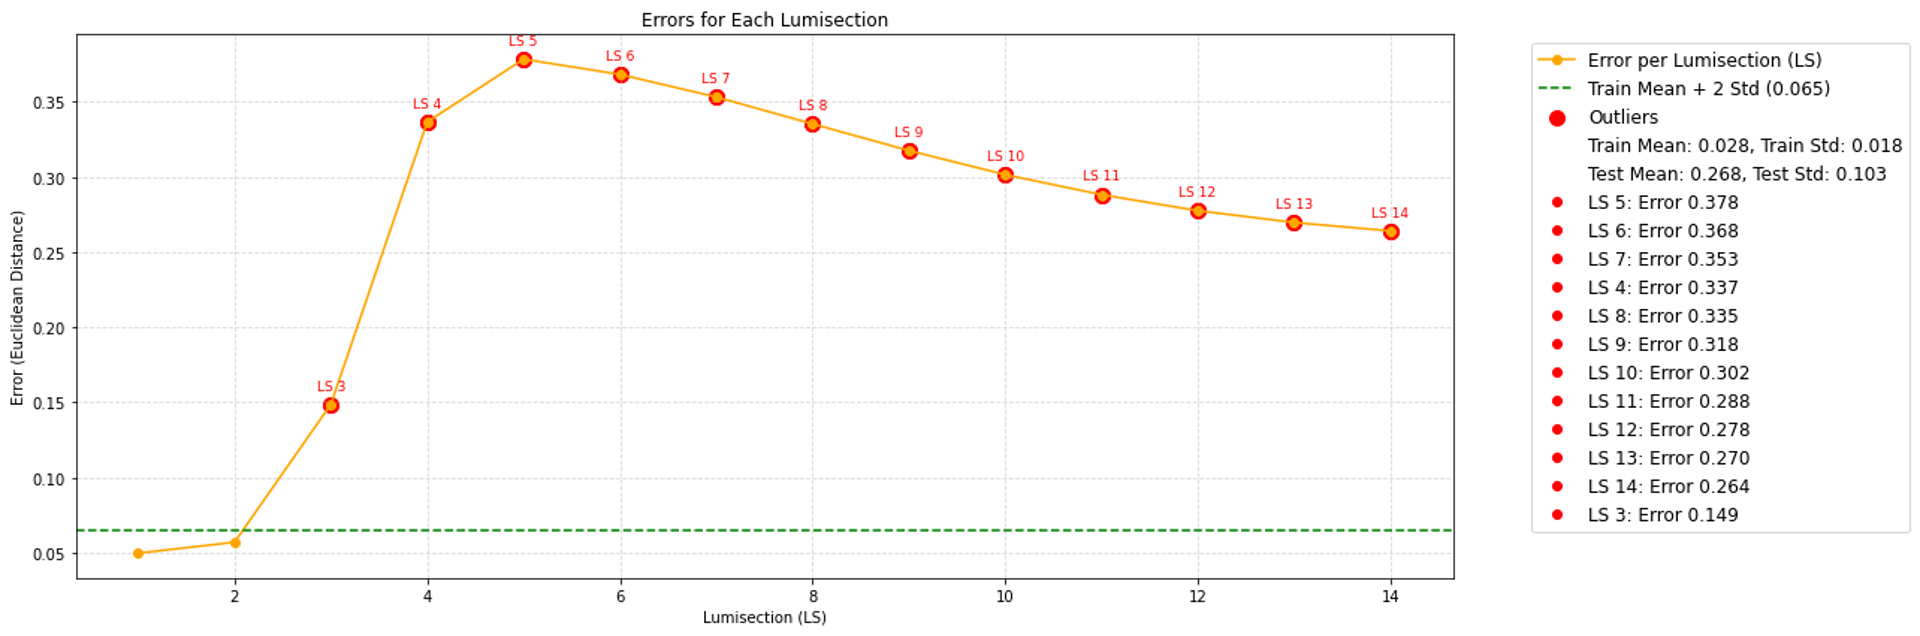
\includegraphics[width=\textwidth]{images/euclid_test_fake.png}
    \end{subfigure}
    \caption{Something.}
    \label{fig:euc_distance}
\end{figure}

\begin{figure}[H]
    \centering
    \begin{subfigure}[t]{1\textwidth}
        \centering
        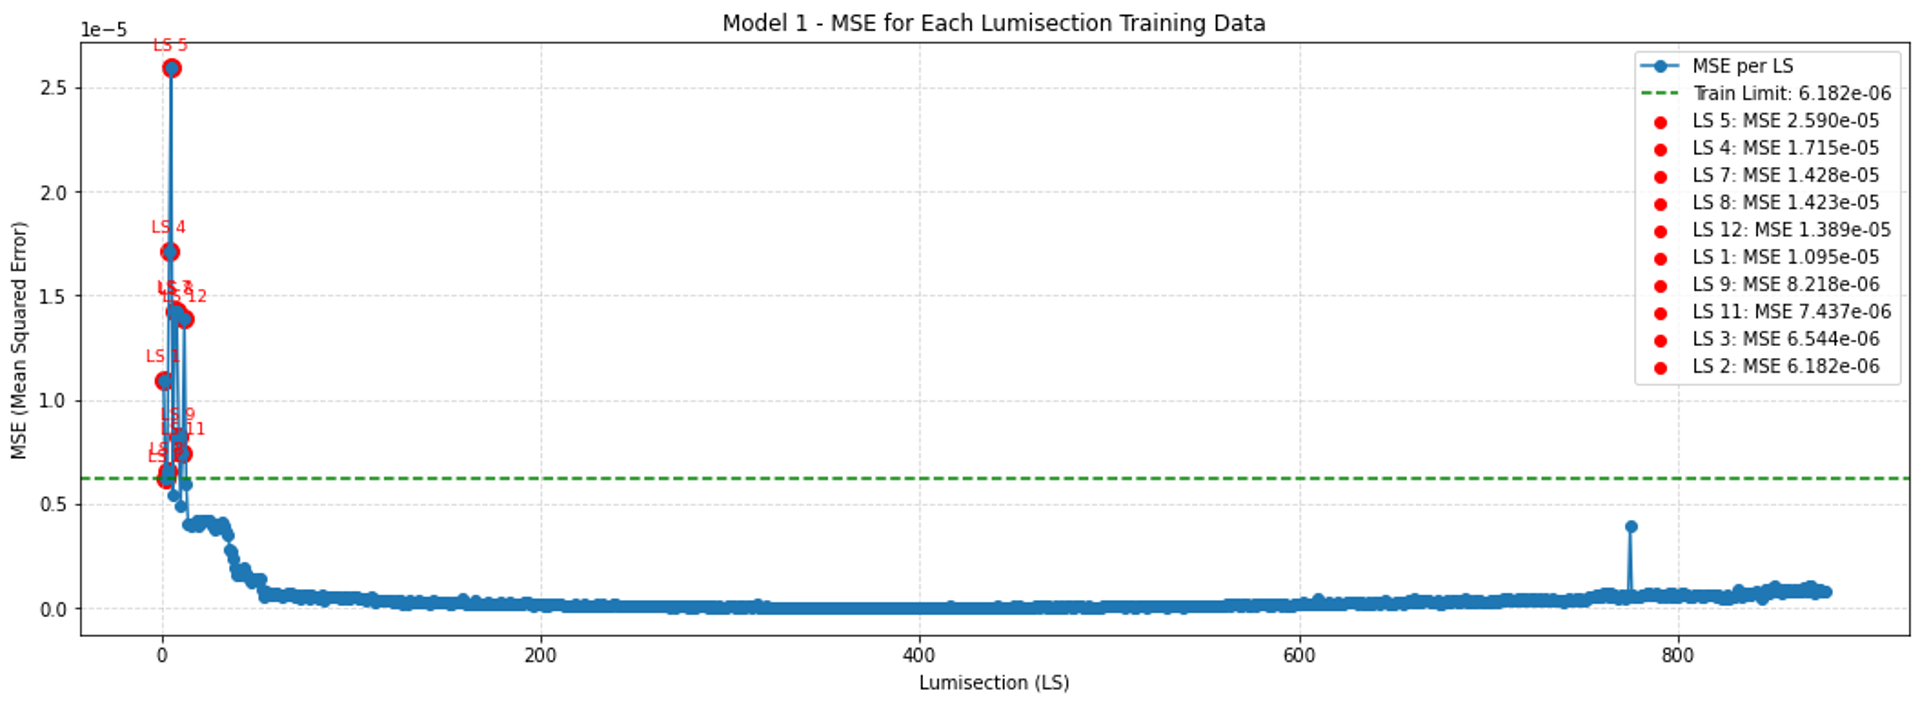
\includegraphics[width=\textwidth]{images/MSE_train.png}
    \end{subfigure}
    \hfill
    \begin{subfigure}[t]{1\textwidth}
        \centering
        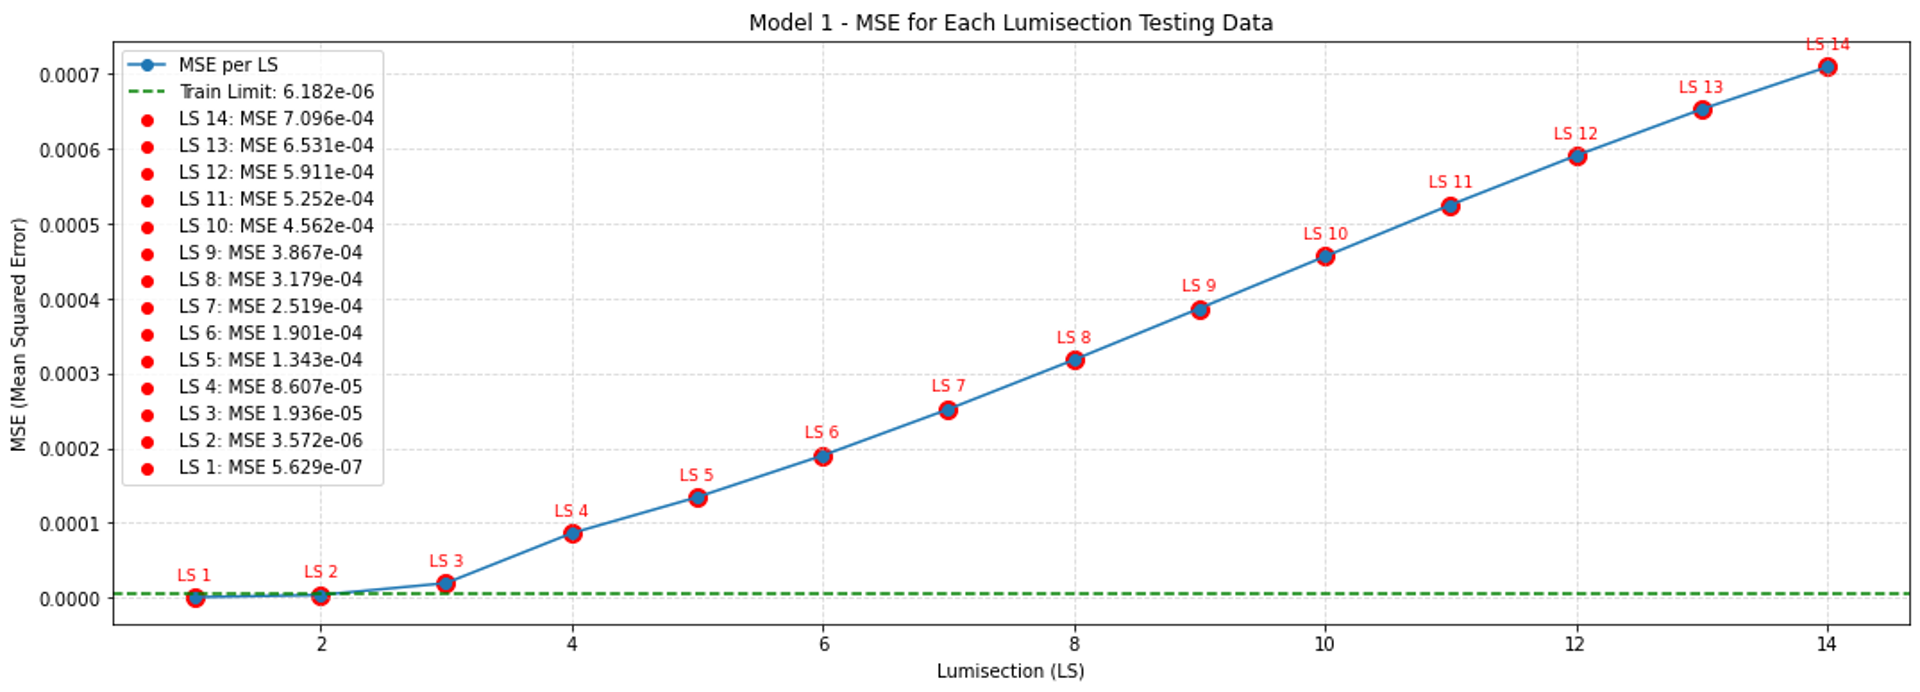
\includegraphics[width=\textwidth]{images/MSE_test.png}
    \end{subfigure}
    \caption{MSE.}
    \label{fig:MSE}
\end{figure}
